\chapter{The Complexity of Algorithms} 
This chapter discusses the computational \blue{complexity} of algorithms.  In order to do so it introduces the
\href{http://en.wikipedia.org/wiki/O_notation}{big $\mathcal{O}$ notation}, which is a notion that is used to
describe the \blue{growth} of a function.  
This  notation is needed when analysing the running time of algorithms.  Furthermore, the big $\mathcal{O}$
notation is part of the technical language of computer science and hence you need to understand this notation
when conversing with your colleagues.

In order to illustrate the application of these notations, we will show how to implement the computation of
powers efficiently, i.e.~we discuss how to evaluate the expression $a^b$ for given $a,b \in \mathbb{N}$ in a way that
is significantly faster than the naive approach.  After that, we discuss the \blue{master theorem}, which
enables us to estimate the \blue{growth rate} of functions that are defined recursively.  Finally, we learn how to solve
\blue{recurrence relations}.  These are recursive equations that arise from the complexity analysis of
functions that are defined recursively.

\section{Motivation}
Sometimes it is necessary to have a precise understanding of the complexity of an algorithm.  
In order to obtain this understanding we could proceed as follows:  
\begin{enumerate}
\item We implement the algorithm in assembly language.
\item We count how many additions, multiplications, assignments, etc.~are needed
      for an input of a given size.  Additionally, we have to count all storage accesses.
\item We look up the amount of time that is needed for the different operations in the processor handbook.
\item Using the information discovered in the previous two steps we predict the running
      time of our algorithm for given input.
\end{enumerate}
This approach is problematic for a number of reasons.
\begin{enumerate}[(a)]
\item It is very complicated and therefore far too time-consuming.
\item The execution time of the basic operations is highly dependent on the memory hierarchy of the
      computer system:  For many modern computer architectures, adding two numbers that happen to be
      in a \blue{register} is more than ten times faster than adding two numbers that reside in
      \blue{main memory}.  Unless we peek into the machine code generated by our compiler, it is very difficult
      to predict whether a variable will be stored in memory or in a register.  Even if a variable
      is stored in main memory, we still might get lucky if the variable is also stored in a \blue{cache}.
\item If we would later code the algorithm in a different programming language or if we would port
      the program to a computer with a different processor we would have to redo most of the
      computation. 
\end{enumerate}
This final reason shows that the approach sketched above is not well suited to measure the complexity of
an \blue{algorithm}: After all, the notion of an algorithm is more abstract than the notion of a program
and we really need a notion measuring the complexity of an algorithm that is more abstract than the
notion of the running time of a program.  This notion of complexity should satisfy the following
specification:

\begin{figure}[t]
  \centering
  \framebox{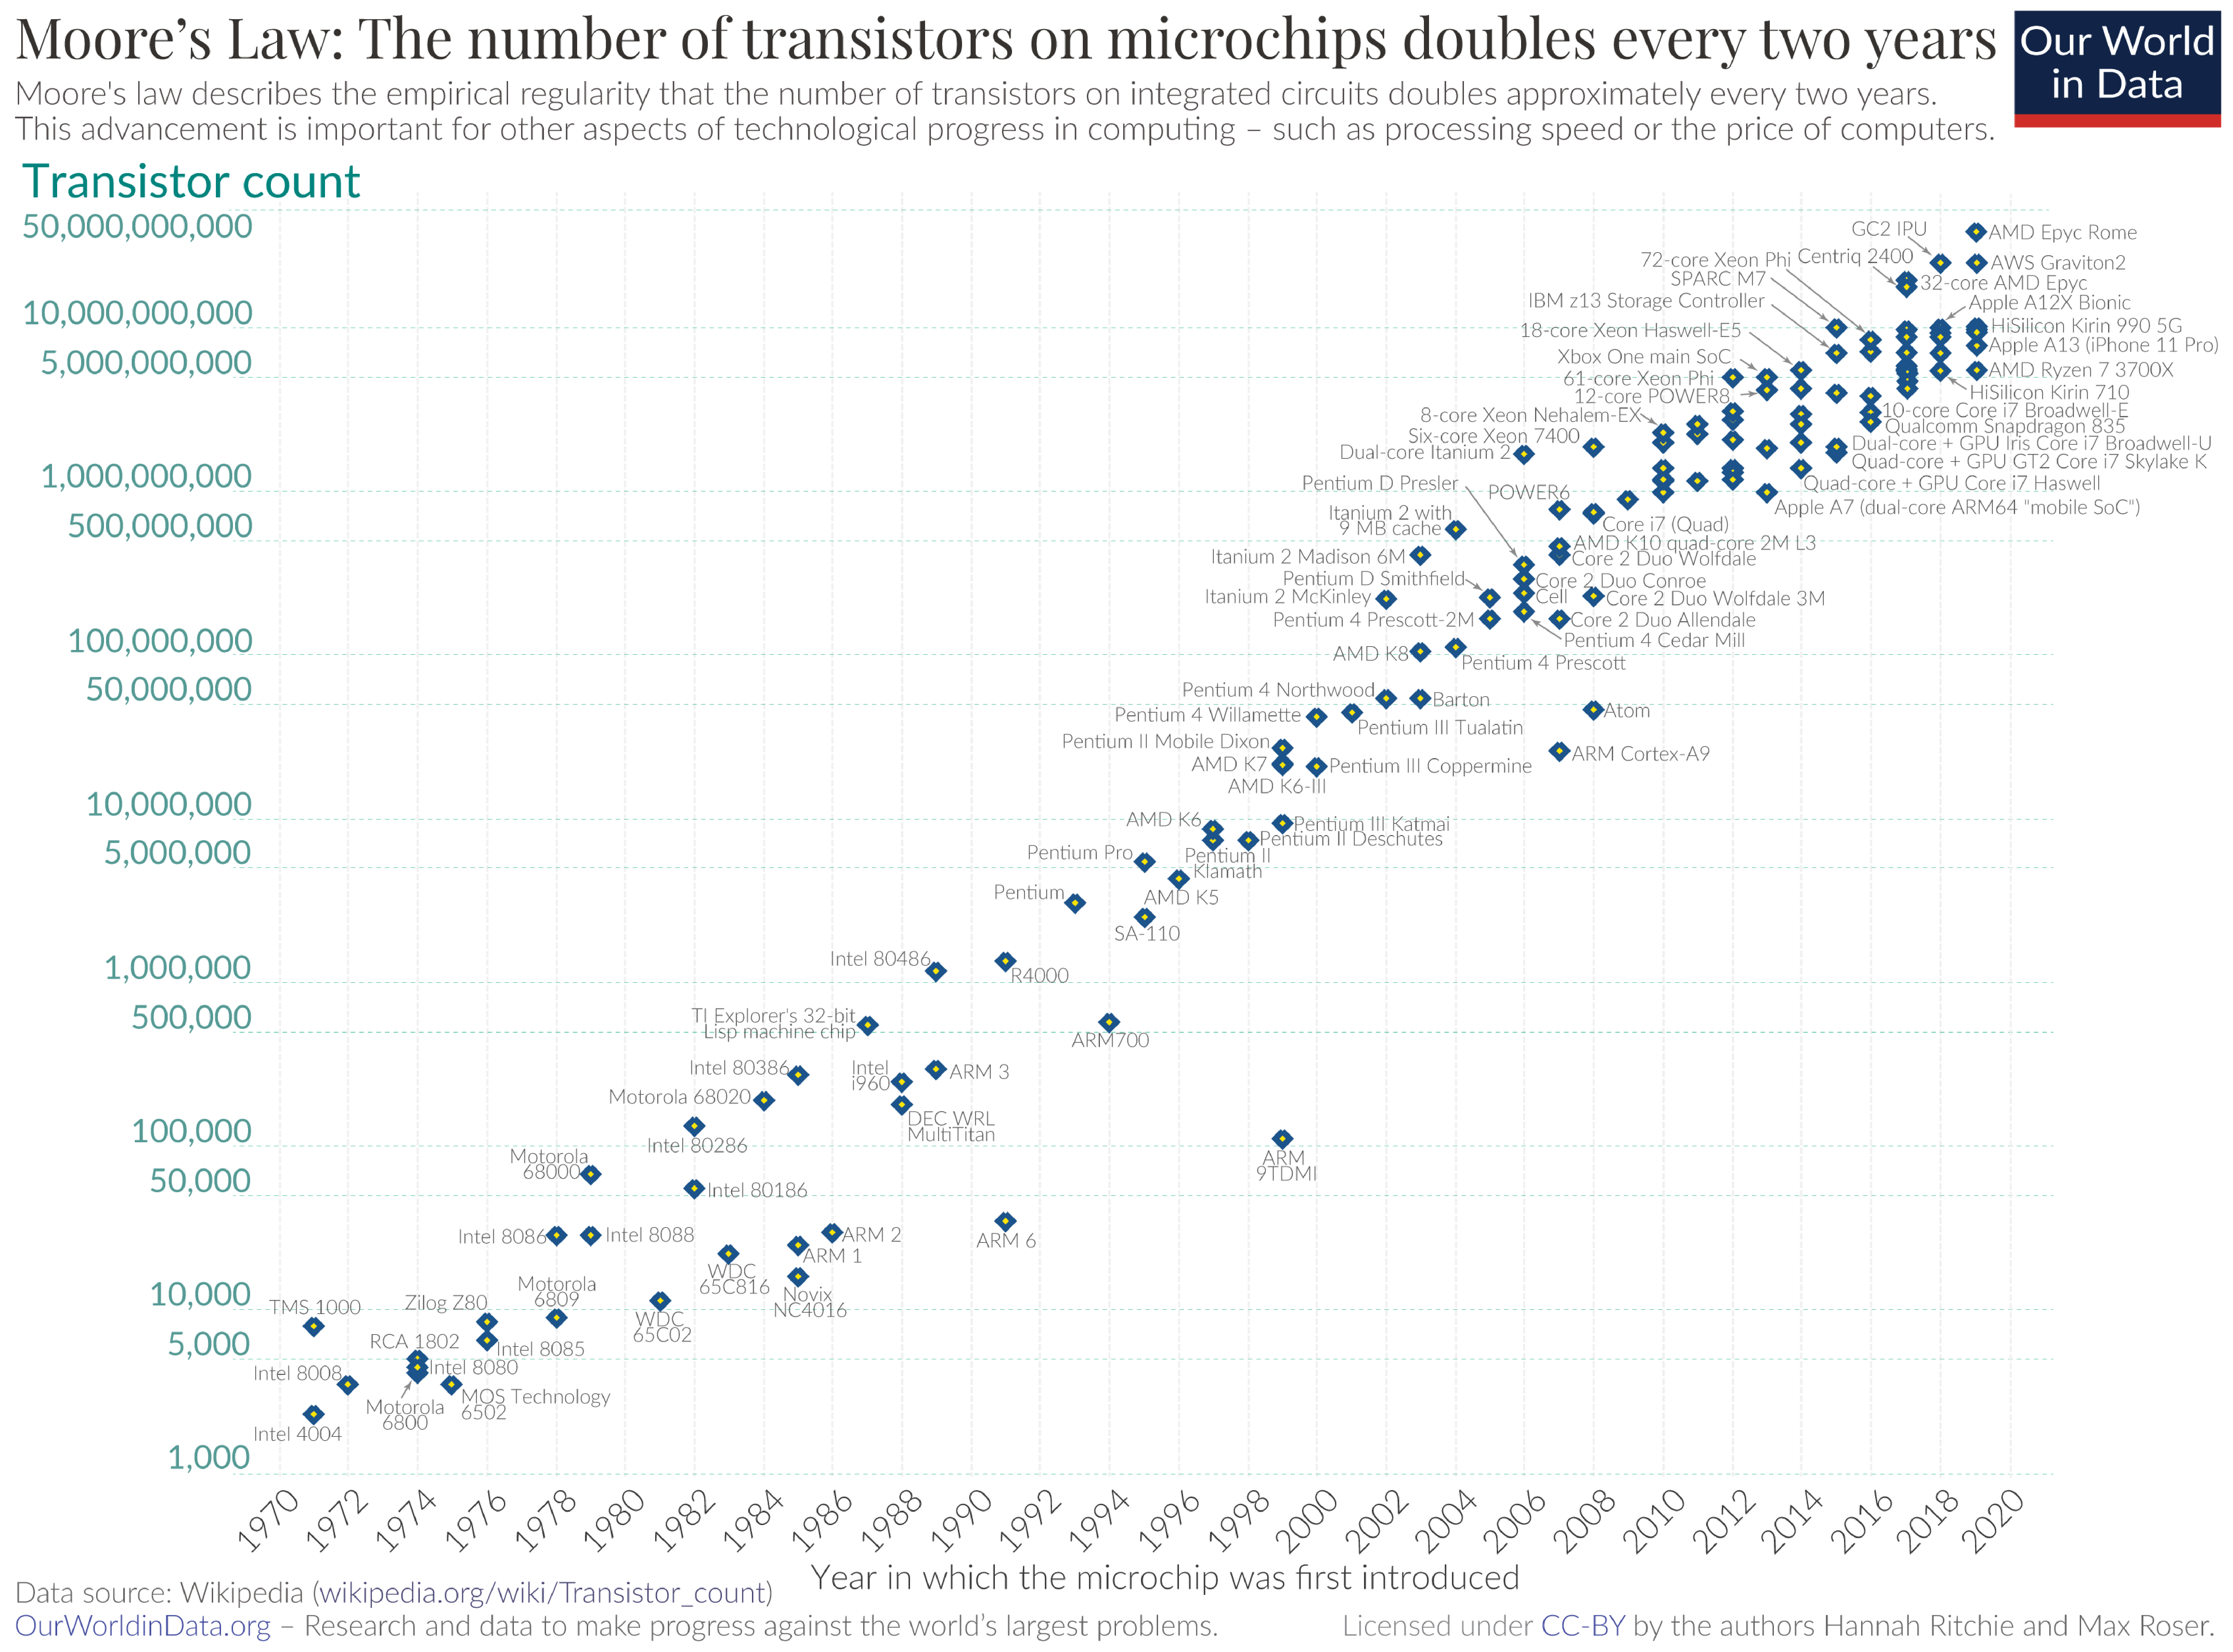
\epsfig{file=Abbildungen/moore.pdf, scale=0.133}} 
  \caption{Moore's Law.} 
  \label{fig:moore.eps}
\end{figure}

\begin{itemize}
\item The notion of complexity should \blue{abstract from constant factors}.  After all, according to 
      \href{http://en.wikipedia.org/wiki/Moore's_law}{Moore's law}, 
      computers hitting the market two years from now will be about twice as powerful as today's computers.
      Figure \ref{fig:moore.eps} on page \pageref{fig:moore.eps} shows Moore's law graphically.
      \FloatBarrier
\item The notion should abstract from \blue{insignificant terms}.

      Assume you have written a program that  multiplies two $n \times n$ matrices.  Assume,
      furthermore, that you have computed the running time $T(n)$ of this program as a function 
      of the size $n$ of the matrix as
      \\[0.2cm]
      \hspace*{1.3cm} $T(n) = 3 \cdot n^3 + 2 \cdot n^2 + 7$. 
      \\[0.2cm]
      When compared with the total running time, the portion of running time that is due to the term 
      $2\cdot n^2 + 7$ will decrease with increasing value of $n$.  To see this, consider the
      following table:
      \\[0.3cm]
      \hspace*{1.3cm} 
      \begin{tabular}{|r|r|}
        \hline
        $n$  & \rule{0pt}{16pt} $\bruch{2 \cdot n^2 + 7}{3 \cdot n^3 + 2 \cdot n^2 + 7}$ \\[0.3cm]
        \hline
        \hline
        1       &  0.75000000000000  \\
        10      &  0.06454630495800  \\
        100     &  0.00662481908150  \\
        1000    &  0.00066622484855  \\
        10\,000 &  6.6662224852\,e\,-05  \\
       \hline
      \end{tabular}

      This table clearly shows that, for large values of $n$, the term $2 \cdot n^2 + 7$ can be
      neglected. 
\item The notion of complexity should describe how the running time increases
      when the size of the input increases:  For small inputs, the running time is not very
      important but the question is how the running time \blue{grows} when the size of the input is increased. 
      Therefore the notion of complexity should capture the relation between the input size and the running time.
\end{itemize}
Let us denote the set of all positive real numbers\footnote{
  In the literature, the set of positive real numbers is often denoted as $\mathbb{R}_{>0}$.}
as $\R_+$, i.e.~let us define 
\\[0.2cm]
\hspace*{1.3cm}
$\R_+ := \{ x \in \R \mid x > 0 \}$. \index{$\mathbb{R}_+$}
\\[0.2cm]
Furthermore, the set of all functions defined on  $\N$ yielding a positive real number is defined
as: 
\\[0.2cm]
\hspace*{1.3cm} 
$\R_+^{\;\N} = \bigl\{ f \mid \mbox{$f$ is a function of the form $f: \N \rightarrow \R_+$} \}$. \index{$\mathbb{R}_+^\mathbb{N}$}
Now we are ready to introduce the \href{https://en.wikipedia.org/wiki/Big_O_notation}{big O notation}.

\begin{Definition}[$\Oh(g)$] 
Assume $g \in \R_+^{\N}$ is given.   Let us define the set of all functions that \blue{grow at most as fast}
  as the function $g$ as follows: \index{$\mathcal{O}(g)$}
  \\[0.2cm]
  \hspace*{0.5cm} 
  \colorbox{red}{\framebox{\colorbox{orange}{
  $ \Oh(g) \;:=\; \left\{ f \in \R_+^{\;\N} \mid \exists k \in \N \colon 
    \exists c \in \R_+\colon \forall n \in \N \colon \bigl(n \geq k \rightarrow f(n) \leq c \cdot g(n)\bigr) \right\}$}}}
  \\[0.2cm]
  Let us put this in words: A function $f:\mathbb{N} \rightarrow \mathbb{R}_+$ is an element of the set
  $\Oh(g)$ iff there are constants $k \in \mathbb{N}$ and $c \in \mathbb{R}_+$ such that
  \\[0.2cm]
  \hspace*{1.3cm}
  $f(n) \leq c \cdot g(n)$ \quad provided that $n \geq k$.
  \\[0.2cm]
  In this case we say that \blue{$f$ is $\mathcal{O}(g)$}.
  \eox
\end{Definition}

The definition of $\Oh(g)$ contains three nested quantifiers and may be difficult to understand
when first encountered.  Therefore, let us analyse this definition carefully.  Let us consider a
function $g \in \R_+^\N$.  Informally, we have the following:
\\[0.2cm]
\hspace*{1.3cm}
\colorbox{red}{\framebox{\colorbox{orange}{
   \blue{$f \in \Oh(g)$}  \quad if and only if \quad \blue{$f$ does not grow faster than a multiple of $g$}
}}}
\\[0.2cm]
We proceed to explain the definition of $\Oh(g)$ in more detail.
\begin{enumerate}
\item The fact that $f \in \Oh(g)$ holds does not impose any restriction on small values of $n$.
      After all, the condition
      \\[0.2cm]
      \hspace*{1.3cm}
      $f(n) \leq c \cdot g(n)$
      \\[0.2cm]
      is only required for those values of $n$ that are bigger than or equal to $k$ and the value
      $k$ can be \underline{an}y\hspace*{-0.1cm}\underline{\ } suitable natural number.

      This property shows that the big $\Oh$ notation captures the \blue{growth rate} of functions.
\item Furthermore, $f(n)$ can be bigger than $g(n)$ even for arbitrary values of $n$ 
      but it can only be bigger by a constant factor:  There must be some fixed constant $c$
      such that 
      \\[0.2cm]
      \hspace*{1.3cm}
      $f(n) \leq c \cdot g(n)$
      \\[0.2cm]
      holds for all values of $n$ that are sufficiently big.  This implies that, for example, if $f \in \Oh(g)$
      holds, then the function $2 \cdot f$ will also be in $\Oh(g)$.

      This last property shows that the big $\Oh$ notation \blue{abstracts from constant factors}.
\end{enumerate}
I have borrowed Figure \ref{fig:big-o.eps} below from the \href{http://www.wikipedia.org}{Wikipedia} article on 
\href{http://en.wikipedia.org/wiki/Asymptotic_notation}{asymptotic notation}.  It shows two functions 
$f(x)$ and $c \cdot g(x)$ such that $f \in \Oh(g)$.  Note that the function $f(x)$, which is drawn
in red, is less or equal than $c \cdot g(x)$ for all values of $x$ such that $x \geq k$.  In the
figure, we have $k=5$, since the condition $f(x) \leq c \cdot g(x)$ is satisfied for $x \geq 5$. For
values of $x$ that are less than $k = 5$, sometimes $f(x)$ is bigger than $c \cdot g(x)$ but that does
not matter.  In Figure \ref{fig:big-o.eps} the functions $f(x)$ and $c \cdot g(x)$ are drawn as if they were
functions defined for all positive real numbers.  However, this is only done to support the
visualization of these functions.  In reality, the functions $f$ and $g$ are only defined for
natural numbers.


\begin{figure}[!ht]
  \centering
  \framebox{\epsfig{file=Abbildungen/big-o.eps, scale=0.50}} 
  \caption{Example for $f \in \Oh(g)$.} 
  \label{fig:big-o.eps}
\end{figure}


\noindent
We discuss some concrete examples in order to further clarify the notion $f \in \Oh(g)$.

\example
We claim that the following holds:
\\[0.2cm]
\hspace*{1.3cm}
$3 \cdot n^3 + 2 \cdot n^2 + 7 \in \Oh(n^3)$. 
\ex

\noindent
\textbf{Proof}:  We have to  provide a constant $c\in\mathbb{R}_+$ and another constant $k\in\mathbb{N}$ such that for all $n\in
\N$ satisfying
$n \geq k$ the inequality
\\[0.2cm]
\hspace*{1.3cm} 
$3 \cdot n^3 + 2 \cdot n^2 + 7 \leq c \cdot n^3$
\\[0.2cm]
holds.  Let us define  $k := 1$ and $c := 12$.  Then we may assume that 
\begin{equation}
  \label{eq:u1}
  1\leq n  
\end{equation}
holds and we have to show that this implies 
\begin{equation}
  \label{eq:u2}
  3 \cdot n^3 + 2 \cdot n^2 + 7 \leq 12 \cdot n^3.
\end{equation}
If we take the third power of both sides of the inequality (\ref{eq:u1}), then we see that
\begin{equation}
  \label{eq:u3pre}
  1 \leq n^3.
\end{equation}
holds.  Let us multiply both sides of this inequality with $7$.  We get: 
\begin{equation}
  \label{eq:u3}
  7 \leq 7 \cdot n^3.
\end{equation}
Furthermore, let us multiply the inequality (\ref{eq:u1}) with the term $2\cdot n^2$.  This yields
\begin{equation}
  \label{eq:u4}
  2 \cdot n^2 \leq 2 \cdot n^3.
\end{equation}
Finally, we obviously have
\begin{equation}
  \label{eq:u5}
  3 \cdot n^3 \leq 3 \cdot n^3.
\end{equation}
Adding up the inequalities (\ref{eq:u3}), (\ref{eq:u4}), and (\ref{eq:u5}) shows that \\[0.2cm]
\hspace*{1.3cm} $3 \cdot n^3 + 2 \cdot n^2 + 7 \leq 12 \cdot n^3$ \\[0.2cm]
for all $n \geq 1$ and therefore the proof is complete. \qed

\example
We have  $n \in \Oh(2^n)$. 
\ex

\proof
We have to provide a constant $c \in \mathbb{R}_+$ and a constant $k\in\mathbb{N}$ such that 
\\[0.2cm]
\hspace*{1.3cm}
$ n \leq c \cdot 2^n$ 
\\[0.2cm]
holds for all $n \geq k$.  Let us define $k := 0$ and $c := 1$.  We have to show that \\[0.2cm]
\hspace*{1.3cm} $n \leq 2^n$ \quad holds for all $n \in \N$.
\\[0.2cm]
We prove this claim by induction on $n$.
\begin{enumerate}
\item \textbf{Base case}: $n = 0$

      Obviously, $n = 0 \leq 1 = 2^0 = 2^n$ holds.  
\item \textbf{Induction step}: $n \mapsto n + 1$

      By the induction hypothesis we have 
      \\[0.2cm]
      \hspace*{1.3cm}
      $n \leq 2^n$.    
      \\[0.2cm]
      Furthermore, a trivial induction shows that
      \\[0.2cm]
      \hspace*{1.3cm}
      $1 \leq 2^n$.
      \\[0.2cm]
      Adding these two inequalities yields
      \\[0.2cm]
      \hspace*{1.3cm} $n+1 \leq 2^n + 2^n = 2^{n+1}$. \qed
\end{enumerate} 

\exercise
\begin{enumerate}[(a)]
\item Prove that $n^2 \in \Oh(2^n)$. 
\item Prove that $n^3 \in \Oh(2^n)$.
      \eoxs
% \item Prove that for every $\alpha \in \mathbb{N}$ we have  $n^\alpha \in \Oh(2^n)$. 
      
%       \hint
%       \begin{enumerate}[1.]
%       \item Try to prove the following claim by induction on $\alpha$:  For every $\alpha \in \mathbb{N}$
%             there exists a number $c(\alpha)$ such that
%             \\[0.2cm]
%             \hspace*{1.3cm}
%             $n^\alpha \leq c(\alpha) \cdot 2^n$ \quad holds for all $n \in \mathbb{N}$.
%             \\[0.2cm]
%             In the induction step you will have to prove that there is a number $c(\alpha+1)$ such that
%             \\[0.2cm]
%             \hspace*{1.3cm}
%             $n^{\alpha+1} \leq c(\alpha+1) \cdot 2^n$ \hspace*{\fill} $(*)$
%             \\[0.2cm]
%             holds.  When proving this claim you may assume by induction hypothesis that for all 
%             $\beta \leq \alpha$ there exist numbers $c(\beta)$ such that
%             \\[0.2cm]
%             \hspace*{1.3cm}
%             $n^{\beta} \leq c(\beta) \cdot 2^n$ \quad holds for all $n \in \mathbb{N}$.
%             \\[0.2cm]
%             You can prove the claim $(*)$ via a \blue{side induction} on $n$.
%       \item The \href{https://en.wikipedia.org/wiki/Binomial_theorem}{binomial theorem}\index{binomial theorem}
%             tells
%             us that for all $n \in \mathbb{N}$ and all $a,b \in \mathbb{R}$ the equation
%             \\[0.2cm]
%             \hspace*{1.3cm}
%             $\ds (a+b)^n = \sum\limits_{k=0}^n {n \choose k} \cdot a^k \cdot b^{n-k}$
%             \\[0.2cm]
%             holds.  Here, the expression ${n \choose k}$ is read as \blue{$n$ choose $k$} and is
%             defined for all $n \in \mathbb{N}$ and all $k \in \{0, 1, 2, \cdots, n\}$ as follows:
%             \\[0.2cm]
%             \hspace*{1.3cm}
%             $\ds {n \choose k} \df \frac{n!}{k! \cdot (n-k)!}$.
%             \\[0.2cm]
%             The binomial theorem should be used to expand the term $(n+1)^{\alpha + 1}$ that occurs
%             in the induction step of the side induction.  \eox
%       \end{enumerate}
\end{enumerate}

It would be very tedious if we would have to use induction every time we need to prove that 
$f \in \Oh(g)$ holds for some functions $f$ and $g$.   Therefore, we show a number of properties of the
big $\Oh$ notation next.  These properties will later enable us to prove claims of the form 
$f \in \Oh(g)$ much quicker than by induction.

\begin{Proposition}[Reflexivity of the Big $\Oh$ Notation] \index{reflexivity of big $\Oh$ notation}
  For all functions $f\colon \N \rightarrow {\R_+}$ we have that
  \\[0.2cm]
  \hspace*{1.3cm} $f \in \Oh(f)$ \quad holds. 
\end{Proposition}

\proof
Let us define $k:=0$ and $c:=1$.  Then our claim  follows immediately from the inequality 
\\[0.2cm]
\hspace*{1.3cm}
$\forall n \in \N\colon f(n) \leq f(n)$. \qed

\begin{Proposition}[Stability of the Big $\Oh$ Notation under Multiplication with Constants] \hspace*{\fill} \linebreak
Assume that we have functions  $f,g\colon \N \rightarrow {\R_+}$ and a number $d \in \R_+$.  Then we
have 
\\[0.2cm]
\hspace*{1.3cm}
 $g \in \Oh(f) \rightarrow d \cdot g \in \Oh(f)$.
\end{Proposition}

\proof
The premiss $g \in \Oh(f)$ implies that there are constants $c'\in \R_+$ and $k'\in \N$ 
such that \\[0.2cm]
\hspace*{1.3cm} 
$\forall n \in \N \colon \bigl(n \geq k'  \rightarrow g(n) \leq c' \cdot f(n)\bigr)$ 
\\[0.2cm]
holds.  If we multiply the inequality involving $g(n)$ with $d$, we get \\[0.2cm]
\hspace*{1.3cm} 
$\forall n \in \N \colon\bigl( n \geq k'  \rightarrow d \cdot g(n) \leq d \cdot c' \cdot f(n)\bigr)$ 
\\[0.2cm]
Let us therefore define $k:=k'$ and $c := d \cdot c'$.  Then we have \\[0.2cm]
\hspace*{1.3cm}
$\forall n \in \N \colon \bigl(n \geq k  \rightarrow d \cdot g(n) \leq c \cdot f(n)\bigr)$ 
\\[0.2cm]
and by definition this implies $d \cdot g \in \Oh(f)$. \qed
\vspace*{0.2cm}

\remark 
The previous proposition shows that the big $\Oh$ notation abstracts
from constant factors. 

\begin{Proposition}[Stability of the Big $\Oh$ Notation under Addition]
Assume that $f,g,h \colon \N \rightarrow {\R_+}$. Then we have 
\\[0.2cm]
\hspace*{1.3cm}
$f \in \Oh(h) \wedge g \in \Oh(h) \,\rightarrow\, f + g \in \Oh(h)$.
\end{Proposition}

\proof
The preconditions $f \in \Oh(h)$ and $g \in \Oh(h)$ imply that there are constants $k_1,k_2\in \N$
and $c_1,c_2\in \R_+$ such that both \\[0.2cm]
\hspace*{1.3cm} 
$\forall n \in \N \colon \bigl( n \geq k_1 \rightarrow f(n) \leq c_1 \cdot h(n)\bigr)$ 
\quad and
\\[0.2cm]
\hspace*{1.3cm} 
$\forall n \in \N \colon\bigl( n \geq k_2 \rightarrow g(n) \leq c_2 \cdot h(n)\bigr)$
\\[0.2cm]
holds.  Let us define $k := \max(k_1,k_2)$ and $c:= c_1 + c_2$.  For all $n \in \mathbb{N}$ such
that $n \geq k$ it then follows that both
\\[0.2cm]
\hspace*{1.3cm}
 $f(n) \leq c_1 \cdot h(n)$ \quad and \quad  $g(n) \leq c_2 \cdot h(n)$
\\[0.2cm]
holds.  Adding these inequalities we conclude that 
\\[0.2cm]
\hspace*{1.3cm} $f(n) + g(n) \leq (c_1 + c_2) \cdot h(n) = c \cdot h(n)$
\\[0.2cm]
holds for all $n \geq k$.
\qed

\exercise
Assume that $f_1,f_2,h_1,h_2 \colon \N \rightarrow {\R_+}$.
\begin{enumerate}[(a)]
\item Prove or refute the claim that 
      \\[0.2cm]
      \hspace*{1.3cm}
      $f_1 \in \Oh(h_1) \wedge f_2 \in \Oh(h_2) \,\rightarrow\, f_1 \cdot f_2 \in \Oh(h_1 \cdot h_2)$
      \\[0.2cm]
      holds.  
\item Assume that $f_1,f_2,h_1,h_2 \colon \N \rightarrow {\R_+}$.  Prove or refute the claim that 
      \\[0.2cm]
      \hspace*{1.3cm}
      $f_1 \in \Oh(h_1) \wedge f_2 \in \Oh(h_2) \,\rightarrow\, f_1 / f_2 \in \Oh(h_1 / h_2)$
      \\[0.2cm]
      holds.  \eoxs
\end{enumerate}

\begin{Proposition}[Transitivity of Big $\mathcal{O}$ Notation] \index{transitivity of big $\mathcal{O}$ notation}
Assume $f,g,h \colon \N \rightarrow {\R_+}$. Then we have \\[0.2cm]
\hspace*{1.3cm}
 $f \in \Oh(g) \wedge g \in \Oh(h) \,\rightarrow\, f \in \Oh(h)$.

\end{Proposition}

\proof
The precondition $f \in \Oh(g)$ implies that there exists a $k_1 \in \N$ and a number $c_1 \in \R_+$
such that 
\\[0.2cm]
\hspace*{1.3cm} 
$\forall n \in \N \colon\bigl( n \geq k_1 \rightarrow f(n) \leq c_1 \cdot g(n)\bigr)$ 
\\[0.2cm]
holds, while the precondition $g \in \Oh(h)$ implies the existence of $k_2 \in \N$ and $c_2 \in \R_+$
such that \\[0.2cm]
\hspace*{1.3cm} 
$\forall n \in \N \colon\bigl( n \geq k_2 \rightarrow g(n) \leq c_2 \cdot h(n)\bigr)$ 
\\[0.2cm]
holds.  Let us define $k:= \max(k_1,k_2)$ and $c := c_1 \cdot c_2$.  Then for all $n \in \mathbb{N}$
such that $n \geq k$ we have the following:
\\[0.2cm]
\hspace*{1.3cm}
$f(n) \leq c_1\cdot g(n)$ \quad and \quad $g(n) \leq c_2 \cdot h(n)$. 
\\[0.2cm]
Let us multiply the second of these inequalities with $c_1$.  Keeping the first inequality this yields
\\[0.2cm]
\hspace*{1.3cm}
$f(n) \leq c_1\cdot g(n)$  \quad and \quad $c_1\cdot g(n) \leq c_1\cdot c_2 \cdot h(n)$. 
\\[0.2cm]
The transitivity of the relation $\leq$ immediately implies $f(n) \leq c \cdot h(n)$ for $n \geq k$.  
\qed

\begin{Proposition}[Limit Proposition] \index{limit proposition} \label{limit}
  Assume that $f,g \colon \N \rightarrow {\R_+}$.   Furthermore, assume that the
  \href{https://en.wikipedia.org/wiki/Limit_of_a_sequence}{limit} 
  \\[0.4cm]
  \hspace*{1.3cm}
 $\lim\limits_{n \rightarrow \infty} \bruch{\,f(n)\,}{g(n)}$
  \\[0.2cm]
  exists.  Then we have $f \in \Oh(g)$. 
\end{Proposition}

\proof
Define \\[0.2cm]
\hspace*{1.3cm}
$\lambda := \lim\limits_{n \rightarrow \infty} \bruch{f(n)}{g(n)}$.  
\\[0.2cm]
Since the limit exists by our assumption, we know that
\\[0.2cm]
\hspace*{1.3cm}
$\ds\forall \varepsilon \in \mathbb{R}_+:\exists k \in \mathbb{R}: \forall n \in \mathbb{N}: 
 \biggl(n \geq k \rightarrow \Bigl| \frac{f(n)}{g(n)} - \lambda \Bigr| < \varepsilon \biggr)
$.
\\[0.2cm]
Since this is valid for all positive values of $\varepsilon$, let us define $\varepsilon := 1$. 
Then there exists a number $k \in \N$ such that
for all $n\in \N$ satisfying $n \geq k$ the inequality 
\\[0.2cm]
\hspace*{1.3cm}
$\left| \bruch{f(n)}{g(n)} - \lambda \right| \leq 1$ 
\\[0.2cm]
holds.  Let us multiply this inequality with $g(n)$.  As $g(n)$ is positive, this yields
\\[0.2cm]
\hspace*{1.3cm}
$|f(n) - \lambda \cdot g(n)| \leq g(n)$. 
\\[0.2cm]
The inequality $|a + b| \leq |a| + |b|$, which is a special case of the
\href{https://en.wikipedia.org/wiki/Triangle_inequality}{triangle inequality} for
real numbers, tells us that  
\\[0.2cm]
\hspace*{1.3cm}
$f(n) =    \bigl|f(n)\bigr|
      =    \bigl|f(n) - \lambda \cdot g(n) + \lambda \cdot g(n)\bigr|
      \leq \bigl|f(n) - \lambda \cdot g(n)\bigr| + \lambda \cdot g(n)$ 
\\[0.2cm]
holds.  Combining the previous two inequalities yields
\\[0.2cm]
\hspace*{1.3cm}
$f(n) \leq \bigl|f(n) - \lambda \cdot g(n)\bigr| + \lambda \cdot g(n)
      \leq g(n) + \lambda \cdot g(n)
       =   (1 + \lambda) \cdot g(n)
$.
\\[0.2cm]
Therefore, we define
\\[0.2cm]
\hspace*{1.3cm}
 $c := 1 +  \lambda$
\\[0.2cm] 
and have shown that $f(n) \leq c \cdot g(n)$ holds for all $n \geq k$. \qed
\vspace*{0.3cm}

\noindent
The following examples show how to put the previous propositions to good use.

\example
Assume $k \in \N$.  Then we have
\\[0.2cm]
\hspace*{1.3cm}
 $n^k \in \Oh(n^{k+1})$.
\ex
 
\proof
We have \\[0.2cm]
\hspace*{1.3cm} 
$\lim\limits_{n \rightarrow \infty} \bruch{n^{k}}{n^{k+1}} = \lim\limits_{n \rightarrow   \infty} \bruch{1}{n} = 0$.
\\[0.2cm]
The claim now follows from the limit proposition. 
\qeds

\example
Assume $k \in \N$ and $\lambda \in \R$ where $\lambda > 1$.  Then we have \\[0.2cm]
\hspace*{1.3cm} $n^k \in \Oh(\lambda^n)$.
\ex

\proof  We will show that 
\hspace*{1.3cm} 
\begin{equation}
  \label{eq:star}
  \lim\limits_{n \rightarrow \infty} \bruch{n^{k}}{\lambda^n} = 0  
\end{equation}
is true.  Then the claim is an immediate consequence of the limit proposition. 
According to \href{https://de.wikipedia.org/wiki/Regel_von_de_L%27Hospital}{L'H\^opital's rule}\footnote{Basically, L'H\^opital's rule states that provided the
  limit $\ds \lim\limits_{x \rightarrow \infty} \frac{f'(x)}{g'(x)}$ exists and $g'(x) \not= 0$, we have
  \\
  \hspace*{1.3cm}
  $\ds\lim\limits_{x \rightarrow \infty} \frac{f(x)}{g(x)} = \lim\limits_{x \rightarrow \infty} \frac{f'(x)}{g'(x)}$.
  \\[0.2cm]
  Here $f'$ and $g'$ denote the derivatives of $f$ and $g$. 
  L'H\^opital's rule is discussed in the \href{https://github.com/karlstroetmann/Analysis/blob/master/Skript/analysis.pdf}{lectures on analysis}.
},  
the limit can be computed as follows: \\[0.2cm]
\hspace*{1.3cm} 
$\displaystyle \lim\limits_{n \rightarrow \infty} \bruch{n^{k}}{\lambda^n} =
\lim\limits_{x \rightarrow \infty} \bruch{x^{k}}{\lambda^x} =
\lim\limits_{x \rightarrow \infty} \bruch{\;\frac{\mathrm{d}x^{k}}{\mathrm{d}x}\;}{\frac{\mathrm{d}\lambda^x}{\mathrm{d}x}}$.
\\[0.2cm]
The derivatives can be computed as follows: \\[0.2cm]
\hspace*{1.3cm}
 $\displaystyle \frac{\mathrm{d}x^{k}}{\mathrm{d}x} = k \cdot x^{k-1}$ \quad and \quad 
 $\displaystyle \frac{\mathrm{d}\lambda^{x}}{\mathrm{d}x} = \ln(\lambda) \cdot \lambda^x$. \\[0.2cm]
We compute the second derivative and get \\[0.2cm]
\hspace*{1.3cm}  
$\displaystyle \frac{\mathrm{d}^{2}\,x^{k}}{\mathrm{d}x^2} = k \cdot (k-1) \cdot x^{k-2}$ \quad and \quad 
 $\displaystyle \frac{\mathrm{d}^2\,\lambda^{x}}{\mathrm{d}x^2} = \ln(\lambda)^2 \cdot \lambda^x$. \\[0.2cm]
In the same manner, we compute the $k$-th order derivative and find \\[0.2cm]
\hspace*{1.3cm} 
$\displaystyle \frac{\mathrm{d}^{k}\,x^{k}}{\mathrm{d}x^k} = k \cdot (k-1) \cdot \cdots \cdot 1 \cdot x^{0} = k!$ \quad and \quad 
 $\displaystyle \frac{\mathrm{d}^k\,\lambda^{x}}{\mathrm{d}x^k} = \ln(\lambda)^k \cdot \lambda^x$. \\[0.2cm]
After $k$ applications of L'H\^opital's rule we arrive at the following chain of equations:
\\[0.2cm]
\hspace*{1.3cm} 
$\ds 
\lim\limits_{x \rightarrow \infty} \frac{x^{k}}{\lambda^x} =
\lim\limits_{x \rightarrow \infty} \frac{\ds\;\frac{\mathrm{d}x^{k}}{\mathrm{d}x}\;}{\ds\frac{\mathrm{d}\lambda^x}{\mathrm{d}x}} =
\lim\limits_{x \rightarrow \infty} \frac{\ds\;\frac{\mathrm{d}^2\,x^{k}}{\mathrm{d}x^2}\;}{\ds\frac{\mathrm{d}^2\,\lambda^x}{\mathrm{d}x^2}} =
\cdots$
\\[0.3cm]
\hspace*{2.8cm}
$\ds = 
\lim\limits_{x \rightarrow \infty} \frac{\ds\;\frac{\mathrm{d}^k\,x^{k}}{\mathrm{d}x^k}\;}{\ds\frac{\mathrm{d}^k\,\lambda^x}{\mathrm{d}x^k}} =
\lim\limits_{x \rightarrow \infty} \frac{k!}{\ln(\lambda)^k \lambda^x} =
\frac{k!}{\ln(\lambda)^k} \cdot \lim\limits_{x \rightarrow \infty} \frac{1}{\lambda^x} = 0$ \quad because
$\lambda > 0$.
\\[0.2cm] 
Therefore the limit exists and the claim follows from the limit proposition.
\qed

\remark
This example shows that any polynomial grows slower than any exponential function with a base greater than 1.
\eoxs

\example
We have $\ln(n) \in \Oh(n)$.
\ex

\proof
This claim is again a simple consequence of the limit proposition.  We will use L'H\^opital's rule
to show that we have
\\[0.4cm]
\hspace*{1.3cm} 
$\lim\limits_{n \rightarrow \infty} \bruch{\;\ln(n)\;}{n} = 0$.
\\[0.2cm]
In the \href{https://github.com/karlstroetmann/Analysis/blob/master/Skript/analysis.pdf}{lecture on analysis}
it is shown that \\[0.2cm] 
\hspace*{1.3cm} $\displaystyle \frac{\mathrm{d} \ln(x)}{\mathrm{d}x} = \frac{1}{x}$ 
\quad and \quad
 $\displaystyle \frac{\mathrm{d} x}{\mathrm{d}x} = 1$. \\[0.2cm]
Therefore, we have \\[0.2cm]
\hspace*{1.3cm} 
$\displaystyle \lim\limits_{n \rightarrow \infty} \bruch{\;\ln(n)\;}{n} = 
\lim\limits_{x \rightarrow \infty} \frac{1/x}{1} = 
\lim\limits_{x \rightarrow \infty} \frac{1}{x} = 0$. \qed


\exercise
Prove that $\sqrt{n} \in \Oh(n)$ holds.  \eox

\exercise
Assume $\varepsilon \in \mathbb{R}$ and $\varepsilon > 0$.  Prove that $\ln(n) \in
\Oh\bigl(n^{\varepsilon}\bigr)$ holds. \eox

\example
We have $2^n \in \Oh(3^n)$, but  $3^n \notin \Oh(2^n)$.
\ex

\proof
 First, we have \\[0.2cm]
\hspace*{1.3cm} 
$\displaystyle\lim\limits_{n \rightarrow \infty} \bruch{2^n}{3^n} = 
 \lim\limits_{n \rightarrow \infty} \left(\bruch{2}{3}\right)^n = 0$
\\[0.2cm]
and the limit proposition therefore shows that $2^n \in \Oh\bigl(3^n\bigr)$.  The proof that $3^n \notin
\Oh(2^n)$ is a  proof\linebreak
\href{https://en.wikipedia.org/wiki/Proof_by_contradiction}{by contradiction}.  Assume that 
$3^n \in \Oh(2^n)$ holds.  Then, there have to be numbers $c$ and $k$ such that 
\\[0.2cm]
\hspace*{1.3cm}
$3^n \leq c \cdot 2^n$ \quad holds for $n \geq k$. 
\\[0.2cm]
Taking the logarithm of both sides of this inequality we find 
\\[0.2cm]
\hspace*{1.3cm}
$
\begin{array}{llcl}
                & \ln(3^n) & \leq & \ln(c \cdot 2^n) \\[0.2cm]
\Leftrightarrow\quad &  n \cdot \ln(3) & \leq & \ln(c) + n \cdot \ln(2) \\[0.2cm]
\Leftrightarrow &  n \cdot \bigl(\ln(3) - \ln(2)\bigr) & \leq & \ln(c)  \\[0.2cm]
\Leftrightarrow &  n  & \leq & \bruch{\ln(c)}{\ln(3) - \ln(2)}          \\[0.2cm]
\end{array}
$
\\[0.2cm]
The last inequality would have to hold for all natural numbers $n$ that are bigger than $k$.  Obviously,
this is not possible as, no matter what value $c$ takes, there are natural numbers $n$ that are bigger than 
\\[0.2cm]
\hspace*{1.3cm}
$\bruch{\ln(c)}{\ln(3) - \ln(2)}$.
\qed

\exercise
\begin{enumerate}[(a)]
\item Assume that $b > 1$.  Prove that $\log_{b}(n) \in \Oh(\ln(n))$.

      \solution
      By the definition of the natural logarithm for any positive number $n$ we have that
      \\[0.2cm]
      \hspace*{1.3cm}
      $n = \mathrm{e}^{\ln(n)}$, \quad where
      \href{http://en.wikipedia.org/wiki/E_(mathematical_constant)}{$\mathrm{e}$} denotes
      \href{https://en.wikipedia.org/wiki/Leonhard_Euler}{Euler's} number. 
      \\[0.2cm]
      Therefore, we can rewrite the expression $\log_b(n)$
      as follows:
      \\[0.2cm]
      \hspace*{1.3cm}
      $
      \begin{array}[t]{lcl}
        \log_b(n) & = & \log_b\bigl(\mathrm{e}^{\ln(n)}\bigr) \\[0.2cm]
                  & = & \ln(n) \cdot \log_b(\mathrm{e})      \\[0.2cm]
                  & = & \log_b(\mathrm{e}) \cdot \ln(n)
      \end{array}
      $
      \\[0.2cm]
      This shows that the logarithm with respect to some base $b$ and the natural logarithm 
      only differ by a constant factor, namely $\log_b(\mathrm{e})$.  Since the big $\mathcal{O}$ notation abstracts from
      constant factors, we conclude that
      \\[0.2cm]
      \hspace*{1.3cm}
      $\log_{b}(n) \in \Oh(\ln(n))$
      \\[0.2cm]
      holds. \qed

      \remark
      The previous exercise shows that, with respect to the big $\mathcal{O}$ notation, the base of
      a logarithm is not important because if $b > 1$ and $c > 1$, then $\log_{b}(n)$ and $ \log_{c}(n)$
      only differ by a constant factor.
\item Prove $\bigl(\log_2(n)\bigr)^2 \in \Oh(n)$.
\item Prove  $\log_2(n) \in \Oh\left(\sqrt{n}\right)$.
\item Assume that $f, g \in \mathbb{R}_+^\mathbb{N}$ and that, furthermore, $f \in \Oh(g)$.  
      Refute the claim that this implies 
      \\[0.2cm]
      \hspace*{1.3cm}
      $\displaystyle 2^{f(n)} \in \Oh\bigl(2^{g(n)}\bigr)$. \eox
\end{enumerate}
% \item Assume that $f, g \in \mathbb{R}_+^\mathbb{N}$ and that, furthermore, 
%       $\lim\limits_{n \rightarrow \infty} \bruch{f(n)}{g(n)} = 0$.  
%       holds.
%       Prove that this implies
%       \\[0.2cm]
%       \hspace*{1.3cm}
%       $\displaystyle 2^{f(n)} \in \Oh\bigl(2^{g(n)}\bigr)$.
% \item Prove that $n^n \in \mathcal{O}\bigl(2^{2^n}\bigr)$.
    
\remark      
It is possible to show that
\\[0.2cm]
\hspace*{1.3cm}
$n^k \in \Oh\bigl(n^{\ln(n)}\bigr)$ \quad for all $k \in \mathbb{N}$
\\
and that
\\
\hspace*{1.3cm}
$n^{\ln(n)} \in \Oh\bigl(b^n\bigr)$ \quad for all $b > 1$.  
\\[0.2cm]
This shows that there are functions that grow faster than any polynomial
function but slower than any exponential function. \eox


\section{A Remark on Notation}
Technically, for some function $g:\mathbb{N} \rightarrow \mathbb{R}_+$ the expression $\Oh(g)$
denotes a set of functions.  Therefore, for a given function $f:\mathbb{N} \rightarrow \mathbb{R}_+$ we can
either have
\\[0.2cm]
\hspace*{1.3cm}
$f \in \Oh(g)$ \quad or \quad $f \not\in \Oh(g)$,
\\[0.2cm]
but we can never have $f = \Oh(g)$.  Nevertheless, in the literature it has become common to abuse the
notation and write
\\[0.2cm]
\hspace*{1.3cm}
$f = \Oh(g)$ \quad instead of \quad $f \in \Oh(g)$.
\\[0.2cm]
You should be aware of the fact that
this abuse of notation is quite dangerous.  For example, if we have two different functions $f_1$ and
$f_2$ such that both
\\[0.2cm]
\hspace*{1.3cm}
$f_1 \in \Oh(g)$ \quad and \quad $f_2 \in \Oh(g)$
\\[0.2cm]
holds, when we would write this as
\\[0.2cm]
\hspace*{1.3cm}
$f_1 = \Oh(g)$ \quad and \quad $f_2 = \Oh(g)$,
\\[0.2cm]
then we must not conclude that $f_1 = f_2$ as the functions $f_1$ and $f_2$ are merely members of
the same set $\Oh(g)$ and are not necessarily equal.  For example, $n \in \Oh(n)$ and 
$2 \cdot n \in \Oh(n)$,  but $n \not= 2 \cdot n$.

For given functions $f$, $g$, and $h$ we write
\\[0.2cm]
\hspace*{1.3cm}
$f = g + \Oh(h)$
\\[0.2cm]
to express the fact that  $\mytt{abs}(f - g) \in \Oh(h)$.  For example, we have 
\\[0.2cm]
\hspace*{1.3cm}
$\ds n^2 + \log_2(n) + n = n^2 + \Oh\bigl(n \cdot \log_2(n)\bigr)$.
\\[0.2cm]
This is true because
\\[0.2cm]
\hspace*{1.3cm}
$\ds \log_2(n) + n \in \Oh\bigl(n \cdot \log_2(n)\bigr)$.
\\[0.2cm] 
The notation $f = g + \Oh(h)$ is useful because it is more precise than the pure big $\Oh$
notation.  For example, assume we have two algorithms $A$ and $B$ for sorting a list of length
$n$.  Assume further that the number $\textsl{count}_A(n)$ of comparisons used by algorithm $A$ to sort a list of
length $n$ is given as
\\[0.2cm]
\hspace*{1.3cm}
$\ds\textsl{count}_A(n) = n \cdot \log_2(n) + n$,
\\[0.2cm]
while for algorithm $B$ the corresponding number of comparisons is given as
\\[0.2cm]
\hspace*{1.3cm}
$\ds\textsl{count}_B(n) = 3 \cdot n \cdot \log_2(n) + n$.
\\[0.2cm]
Then the big $\Oh$ notation is not able to distinguish between the complexity of algorithm $A$ and
algorithm $B$ since we have
\\[0.2cm]
\hspace*{1.3cm}
$\textsl{count}_A(n) \in \Oh\bigl(n \cdot \log_2(n)\bigr)$ \quad as well as \quad
$\textsl{count}_B(n) \in \Oh\bigl(n \cdot \log_2(n)\bigr)$.
\\[0.2cm]
However, by writing
\\[0.2cm]
\hspace*{1.3cm}
$\ds\textsl{count}_A(n) = n \cdot \log_2(n) + \Oh(n)$ \quad and \quad
$\ds\textsl{count}_B(n) = 3 \cdot n \cdot \log_2(n) + \Oh(n)$
\\[0.2cm]
we can abstract from lower order terms while still retaining the leading coefficient of the term
determining the complexity.  

\section[Computation of Powers]{Case Study:  Efficient Computation of Powers}
\index{computation of powers}
Let us study an example to clarify the notions introduced so far.  
Consider the program shown in Figure \ref{fig:power-naive.stlx}.  Given an integer $m$ and a
natural number $n$, $\mytt{power}(m, n)$ computes the value $m^n$.
The basic idea is to compute the value of $m^n$ according to the formula \\[0.2cm]
\hspace*{1.3cm} 
$m^n = \underbrace{m \cdot {\dots} \cdot m}_n$. 


\begin{figure}[!h]
  \centering
\begin{python3code}
    def power(m, n):
        r = 1
        for i in range(n):
            r = r * m
        return r
\end{python3code}
\vspace*{-0.7cm}
  \caption{Naive computation of $m^n$ for  $m,n \in \N$.}
  \label{fig:power-naive.stlx}
\end{figure} 
 
This program is obviously correct.  The computation of $m^n$ requires $n$ multiplications if the
function \mytt{power}  is implemented as shown in Figure \ref{fig:power-naive.stlx}.
Fortunately, there is an algorithm for computing $m^n$ that is much more efficient.
This algorithm is known as iterative squaring or as
\href{https://en.wikipedia.org/wiki/Exponentiation_by_squaring}{exponentiation by squaring}.
\index{iterative squaring} 
Consider we have to evaluate $m^4$.  We have
 \\[0.2cm]
\hspace*{1.3cm} 
$m^4 = (m \cdot m) \cdot (m \cdot m)$.
\\[0.2cm]
If the expression $m\cdot m$ is computed just once, the computation of
$m^4$ requires only two multiplications while the naive approach would already use 3 multiplications.
In order to compute $m^8$ we can proceed according to the following formula: \\[0.2cm]
\hspace*{1.3cm} 
$m^8 = \bigl( (m \cdot m) \cdot (m \cdot m) \bigr) \cdot \bigl( (m \cdot m) \cdot (m \cdot m)
\bigr)$. 
\\[0.2cm]
If the expression $(m \cdot m) \cdot (m \cdot m)$ is computed only once, then we need just 3 multiplications
in order to compute $m^8$.   On the other hand, the naive approach would take 7 multiplications to
compute $m^8$.  The general case is implemented in the program shown in Figure \ref{fig:power.stlx}.  
In this program, the value of $m^n$ is computed according to the 
\href{http://en.wikipedia.org/wiki/Divide_and_conquer_algorithm}{divide and conquer} \index{divide and conquer}
paradigm.  The basic idea that makes this program work is captured by the following formula: 
\\[0.2cm] 
\hspace*{1.3cm} 
$m^n = 
\left\{\begin{array}{ll}
m^{n\dvv 2} \cdot m^{n\dvv 2}          & \mbox{if $n$ is even};    \\
m^{n\dvv 2} \cdot m^{n\dvv 2} \cdot m  & \mbox{if $n$ is odd}.
\end{array}
\right.
$
\\[0.2cm]
In this formula $n \dv  2$ denotes \blue{integer division} by $2$, e.g.~we have $4 \dv  2 = 2$, but also
$5 \dv  2 = 2$.
In general, if $a,b \in \mathbb{N}$ and $b > 0$, it can be shown that there exist natural numbers $q$ and $r$
such that
\\[0.2cm]
\hspace*{1.3cm}
$a = b \cdot q + r$ \quad where $0 \leq r < b$. \hspace*{\fill} (ID)
\\[0.2cm]
Furthermore, $q$ and $r$ are uniquely determined by the condition (ID).  Then, $q$ is called the \blue{integer division} 
of $a$ by $b$ and $r$ is called the \blue{remainder} of the integer division of $a$ by $b$ and we write
\\[0.2cm]
\hspace*{1.3cm}
$q = a \mbox{\,\mytt{/}$\!$\mytt{/}\,} b$ \quad and \quad $r = a \;\mytt{\%}\; b$.
\ex

\begin{figure}[!h]
  \centering
\begin{python3code} 
    def power(m, n):
        if n == 0:
            return 1
        p = power(m, n // 2)
        if n % 2 == 0:
            return p * p
        else:
            return p * p * m
\end{python3code}
\vspace*{-0.7cm}
  \caption{Computation of $m^n$ for $m,n \in \N$.}
  \label{fig:power.stlx}
\end{figure} 

Next, we want to analyse the \blue{computational complexity} of our implementation of \mytt{power}.
To this end, let us compute the number of multiplications that are performed when
$\mytt{power}(m,n)$ is called.  If the number $n$ is odd there will be more multiplications than
in the case when $n$ is even.  Let us first investigate the \blue{worst case}.  
The worst case happens if there is an $l\in \N$ such that 
\\[0.2cm]
\hspace*{1.3cm}
$n = 2^l - 1$. 
\\[0.2cm]
The reason is that then
\\[0.2cm]
\hspace*{1.3cm} $n \dv 2 = 2^{l-1} - 1$
\\[0.2cm]
and hence $n \dv 2$ is of the same form as $n$ and, in particular, is odd again.  To see this, note that
for $n = 2^l - 1$ we have that
\\[0.2cm]
\hspace*{1.3cm}
$2 \cdot(n \dv 2) + n \,\mytt{\symbol{37}}\, 2 = 2 \cdot (2^{l-1} - 1) + 1 = 2^l - 1 = n$,
\\[0.2cm]
showing that $(2^l -1 ) \dv 2 = 2^{l-1} -1$.
Therefore, if $n = 2^l - 1$ the exponent $n$ will be odd on every recursive call until it finally reaches $0$.
Let us assume $n = 2^l - 1$ and let us compute the number $a_n$ of multiplications that
are done when $\mytt{power}(m,n)$ is evaluated:
\\[0.2cm]
\hspace*{1.3cm}
$a_n := \mbox{number of multiplications to compute \mytt{power}}(m, n)$.
\\[0.2cm]
First, we have $a_0 = 0$, because if we have $n = 2^0 - 1 = 0$, then the evaluation of 
$\mytt{power}(m, n)$ does not require a single multiplication.
Otherwise, we have two multiplications in line 8 that have to be added to those multiplications
that are performed in the recursive call in line 4.  Therefore, we get the following
\href{http://en.wikipedia.org/wiki/Recurrence_relation}{recurrence relation}\footnote{
  A \blue{recurrence relation} \index{recurrence relation} for a sequence $a_n$ is any equation that relates
  $a_n$ to preceding terms of the sequence $a_n$.  For example, $a_n = a_{n-1} + 1$ for $n > 0$ is a very
  simple recurrence relation, while $a_n = a_{n \dv 2} + n$ for $n > 0$ is a more complicated recurrence
  relation.  In order for a recurrence relation to \blue{define} the sequence $a_n$ we also need to specify one
  or more initial values.  
}:
\\[0.2cm]
\hspace*{1.3cm}
$a_n = a_{n \dvv 2} + 2$ \qquad for all $n \in \left\{2^l - 1 \mid l \in \N\right\}$\quad and $a_0 = 0$. 
\\[0.2cm]
In order to solve this recurrence relation, let us define $b_l := a_{2^l-1}$.  Then, the sequence
$(b_l)_l$ 
satisfies the recurrence relation
 \\[0.2cm]
\hspace*{1.3cm} 
$\ds b_l = a_{2^l-1} = a_{(2^l-1) \dvv 2} + 2 = a_{2^{l-1}-1} + 2 = b_{l-1} +2$ \qquad for all $l\in\N$ with
$l > 0$
\\[0.2cm]
and the initial term $b_0$ satisfies $b_0 = a_{2^0-1} = a_0 = 0$.  It is quite obvious that the
solution of the recurrence relation $b_l = b_{l-1} + 2$ with initial condition $b_0 = 0$ is given by the formula
\\[0.2cm]
\hspace*{1.3cm} $b_l = 2 \cdot l$ \qquad for all $l \in \N$. 
\\[0.2cm] 
This claim is readily established via a trivial induction.  Plugging in the definition $b_l = a_{2^l-1}$ we
see that the sequence $a_n$ satisfies \\[0.2cm]
\hspace*{1.3cm} $a_{2^l-1} = 2 \cdot l$. 
\\[0.2cm]
Let us solve the equation $n = 2^l - 1$ for $l$.  This yields
 $l =
\log_2(n+1)$.  Substituting this expression in the formula above gives \\[0.2cm]
\hspace*{1.3cm} $a_n = 2 \cdot \log_2(n+1) \in \Oh\bigl(\log_2(n)\bigr)$.
\vspace*{0.3cm}

Next, we consider the best case.  The computation of
$\mytt{power}(m,n)$ needs the least number of multiplications if the test 
\mytt{n \% 2 == 0}
always evaluates as true.  In this case, $n$ has to be a power of $2$.  
Hence there has to exist an $l\in \N$ such that we have
 \\[0.2cm]
\hspace*{1.3cm} $n = 2^l$.
 \\[0.2cm]
Therefore, let us now assume $n = 2^l$ and let us again compute the number $a_n$ of multiplications
that are needed to compute $\mytt{power}(m,n)$. 

First, we have $a_{2^0} = a_1 = 2$, because if $n = 1$, the test \mytt{n \% 2 == 0} fails and in
this case line 8 yields two multiplications.  Furthermore, in this case
line 4 does not add any multiplications since the call $\mytt{power}(m,0)$ immediately returns its
result.

Now, if $n = 2^l$ and $n > 1$ then line 6 yields one multiplication that 
has to be added to those multiplications that are done during the recursive invocation of
\mytt{power} in line 4.  Therefore, we have the following recurrence relation:
 \\[0.2cm]
\hspace*{1.3cm} $a_n = a_{n \dvv 2} + 1$ \qquad for all $n \in \left\{2^l \mid l \in \N\right\}$\quad and
$a_1 = 2$. 
\\[0.2cm]
Let us define $b_l := a_{2^l}$.  Then the sequence $(b_l)_l$ satisfies the recurrence relation
 \\[0.2cm]
\hspace*{1.3cm} 
$b_l = a_{2^l} = a_{2^l \dvv 2} + 1 = a_{2^{l-1}} + 1 = b_{l-1} + 1$ \qquad for all $l\in\N$, \\[0.2cm]
and the initial value is given as $b_0 = a_{2^0} = a_1 = 2$.
Therefore, we have to solve the recurrence relation 
\\[0.2cm]
\hspace*{1.3cm}
 $b_{l+1} = b_l + 1$ \qquad for all $l \in \N$ \quad with $b_0 = 2$.\\[0.2cm]
Obviously, the solution is \\[0.2cm]
\hspace*{1.3cm} $b_l = 2 + l$ \qquad for all $l\in\N$.
\\[0.2cm]
If we substitute this into the definition of $b_l$ in terms of $a_l$ we have: \\[0.2cm]
\hspace*{1.3cm}
$a_{2^l} = 2 + l$. 
\\[0.2cm]
If we solve the equation $n = 2^l$ for  $l$ we get $l =
\log_2(n)$. Substituting this value leads to
\\[0.2cm]
\hspace*{1.3cm}
 $a_n = 2 + \log_2(n) \in \Oh\bigl(\log_2(n)\bigr)$.
\vspace*{0.3cm}

Since we have gotten the same result both in the worst case and in the best case we may conclude
that in general the number $a_n$ of multiplications needed to compute $\mytt{power}(m, n)$ satisfies 
\\[0.2cm]
\hspace*{1.3cm} 
$a_n \in \Oh\bigl(\log_2(n)\bigr)$. \qed

\remark
In reality, we are not interested in the number of multiplications but we are rather interested
in the amount of computation time needed by the algorithm given above.
However, this computation would be much more tedious because then we would have to take into account
that the time needed to multiply two numbers depends on the size of these numbers.

\exercise
Implement a procedure $\mytt{div\_mod}$ that takes two numbers $m$ and $n$ and that returns the pair
\\[0.2cm]
\hspace*{1.3cm}
$\bigl(m \dv n, m \;\mytt{\%}\; n\bigr)$.
\\[0.2cm]
Therefore, if $\mytt{div\_mod}(m, n) = (q,r)$ we will have both
\\[0.2cm]
\hspace*{1.3cm}
$m = n \cdot q + r$ \quad and \quad $0 \leq r < n$.
\\[0.2cm]
You should implement the function recursively and compute 
$\mytt{div\_mod}(m, n)$ by recursively computing $\mytt{div\_mod}(m \dv 2, n)$.
In your implementation of $\mytt{div\_mod}$ you are only permitted to use the operators $\dv$ and
$\mytt{\%}$ when the second argument of these operators is $2$, i.e.~you are permitted to
use the expressions $m \dv 2$ and $m \;\mytt{\%}\; 2$ as these expressions can be implemented
using bit operations.

\exercise
Given a natural number $n$, the \blue{integer square root} \index{integer square root} of $n$ is the largest
number $r$ such that $r^2$ is less or equal than $n$, i.e. we have
\\[0.2cm]
\hspace*{1.3cm}
$\mytt{isqrt}(n) := \max\bigl(\{ r \in \mathbb{N} \mid r^2 \leq n \}\bigr)$.
\begin{enumerate}[(a)]
\item Develop a recursive algorithm that computes $\mytt{isqrt}(n)$ in terms of $\mytt{isqrt}(n\dv4)$.
\item Implement this algorithm in \textsl{Python}.
\end{enumerate}

\section{The Master Theorem}
In order to analyse the complexity of  the procedure $\textsl{power}()$,
we have first computed a  recurrence relation, then we have solved this recurrence and, finally,  
we have approximated the result using the big $\Oh$ notation.  In many cases we are only interested in this
last approximation and in that case it is not necessary to actually solve the recurrence relation.  
Instead, we can use the 
\href{http://en.wikipedia.org/wiki/Master_theorem#Generic_form}{master theorem}\index{master theorem} to short 
circuit the procedure for computing the complexity of an algorithm. 
We present a simplified version of the master theorem next.

\begin{Theorem}[\blue{Master Theorem} \index{Master Theorem}] 
  Assume that 
  \begin{enumerate}[(a)]
  \item $\alpha,\beta \in \mathbb{N}$ such that  $\beta \geq 2$, $\delta \in \mathbb{R}$ such that $\delta \geq
    0$ and
  \item the function $f:\N \rightarrow \R_+$ satisfies the recurrence relation
        \\[0.2cm]
        \hspace*{1.3cm}
        $f(n) = \alpha \cdot f\left(n \dv \beta\right) + \Oh(n^\delta)$,
        \\[0.2cm]
        where $n \dv \beta$ denotes \blue{integer division}\footnote{
          For given integers $a, b \in \mathbb{N}$, the \blue{integer division} $a \dv b$
          is defined as the biggest number $q \in \mathbb{N}$ such that $q \cdot b \leq a$.  
        }  
        of $n$ by $\beta$.
  \end{enumerate}
  Then we have the following:
  \begin{enumerate}
  \item $\alpha < \beta^\delta\rightarrow f(n) \in \Oh\bigl(n^{\delta}\bigr)$,
  \item $\alpha = \beta^\delta\rightarrow f(n) \in \Oh\bigl(\log_\beta(n) \cdot n^{\delta}\bigr)$,
  \item $\alpha > \beta^{\delta} \rightarrow f(n) \in \Oh\bigl(n^{\log_{\beta}(\alpha)}\bigr)$. 
  \end{enumerate}
\end{Theorem}

\proof
We will compute an upper bound for the expression $f(n)$, but in order to keep our exposition clear
and simple we will only discuss the case where $n$ is a power of $\beta$, that is $n$ has the form
\\[0.2cm]
\hspace*{1.3cm}
$n = \beta^k$ \quad for some $k \in \mathbb{N}$.
\\[0.2cm]
The general case is similar, but is technically much more involved.
Observe that the equation $n = \beta^k$ implies $k = \log_{\beta}(n)$.  We will need this equation later. 
Furthermore, in order to simplify our exposition even further, we assume that the recurrence
relation for $f$ has the form 
\\[0.2cm]
\hspace*{1.3cm}
 $f(n) = \alpha \cdot f\left(n \dv \beta\right) + n^\delta$,
\\[0.2cm]
i.e.~instead of adding the term $\Oh\bigl(n^\delta\bigr)$ we just add $n^\delta$.  These
simplifications do not change the proof idea.  Without them, the proof would be much more involved and the main
idea of the proof would be hidden.  We start the proof by defining
\\[0.2cm]
\hspace*{1.3cm}
 $a_k := f(n) = f\bigl(\beta^k\bigr)$.  
\\[0.2cm]
Then the recurrence relation for the function $f$
is transformed into a recurrence relation for the sequence $a_k$ as follows:
\\[0.2cm]
\hspace*{1.3cm}
$
\begin{array}[t]{lcl}
a_k & = & f\bigl(\beta^{k}\bigr)                                             \\[0.2cm]
    & = & \alpha \cdot f\bigl(\beta^{k} \dv \beta\bigr) + \bigl(\beta^{k}\bigr)^\delta    \\[0.2cm]
    & = & \alpha \cdot f\bigl(\beta^{k-1}\bigr) + \beta^{k \cdot \delta}    \\[0.2cm]
    & = & \alpha \cdot a_{k-1} + \beta^{k \cdot \delta}    \\[0.2cm]
    & = & \alpha \cdot a_{k-1} + \bigl(\beta^{\delta}\bigr)^k    \\[0.2cm]
\end{array}
$
\\[0.2cm]
In order to simplify this recurrence relation, let us define
\\[0.2cm]
\hspace*{1.3cm}
$\gamma := \beta^{\delta}$.
\\[0.2cm]
Then, the recurrence relation for the sequence $a_k$ can be written as
\\[0.2cm]
\hspace*{1.3cm}
$a_k = \alpha \cdot a_{k-1} + \gamma^k$.
\\[0.2cm]
Let us substitute $k-1$ for $k$ in this equation.  This yields
\\[0.2cm]
\hspace*{1.3cm}
$a_{k-1} = \alpha \cdot a_{k-2} + \gamma^{k-1}$.
\\[0.2cm]
Next, we plug the value of $a_{k-1}$ into the equation for $a_k$.  This yields
\\[0.2cm]
\hspace*{1.3cm}
$
\begin{array}[t]{lcl}
  a_k & = & \alpha \cdot a_{k-1} + \gamma^k  \\[0.2cm]
      & = & \alpha \cdot \bigl(\alpha \cdot a_{k-2} + \gamma^{k-1}\bigr) + \gamma^k \\[0.2cm]
      & = & \alpha^2 \cdot a_{k-2} + \alpha \cdot \gamma^{k-1} + \gamma^k. \\[0.2cm]
\end{array}
$
\\[0.2cm]
We observe that 
\\[0.2cm]
\hspace*{1.3cm}
$a_{k-2} = \alpha \cdot a_{k-3} + \gamma^{k-2}$
\\[0.2cm]
holds and substitute the right hand side of this equation into the previous equation.  This yields
\\[0.2cm]
\hspace*{1.3cm}
$
\begin{array}[t]{lcl}
  a_k & = & \alpha^2 \cdot a_{k-2} + \alpha \cdot \gamma^{k-1} + \gamma^k
            \\[0.2cm]
      & = & \alpha^2 \cdot \bigl(\alpha \cdot a_{k-3} + \gamma^{k-2}\bigr) + \alpha \cdot \gamma^{k-1} + \gamma^k
            \\[0.2cm]
      & = & \alpha^3 \cdot a_{k-3} + \alpha^2 \cdot \gamma^{k-2} + \alpha^1 \cdot \gamma^{k-1} + \alpha^0 \cdot \gamma^k. 
            \\[0.2cm]
\end{array}
$
\\[0.2cm]
Proceeding in this way we arrive at the general formula
\\[0.2cm]
\hspace*{1.3cm}
$
\begin{array}[b]{lcl}
a_k & = & \alpha^{i} \cdot a_{k-i} + \alpha^{i-1} \cdot \gamma^{k-(i-1)} + \alpha^{i-2} \cdot \gamma^{k-(i-2)}
          + \cdots + \alpha^0 \cdot \gamma^k 
          \\[0.2cm]
    & = & \ds \alpha^{i} \cdot a_{k-i} + \sum\limits_{j=0}^{i-1} \alpha^{j} \cdot \gamma^{k-j}. \\[0.2cm]
\end{array}
$
\\[0.2cm]
If we take this formula and substitute $i := k$, then we conclude
\\[0.2cm]
\hspace*{1.3cm}
$\displaystyle 
\begin{array}[b]{lcl}
a_k & = & \ds\alpha^{k} \cdot a_{0} + \sum\limits_{j=0}^{k-1} \alpha^{j} \cdot \gamma^{k-j} \\[0.5cm]
    & = & \ds\alpha^{k} \cdot a_{0} + \gamma^k \cdot \sum\limits_{j=0}^{k-1} \Bigl(\displaystyle\frac{\,\alpha\,}{\gamma}\Bigr)^j.  \\[0.2cm]
\end{array}
$
\\[0.2cm]
At this point we have to remember the formula for the geometric series.  This formula reads
\\[0.2cm]
\hspace*{1.3cm}
$\displaystyle\sum\limits_{j=0}^n q^j = \bruch{q^{n+1} - 1}{q - 1}$ \quad provided $q \not= 1$, while
\\[0.2cm]
\hspace*{1.3cm}
$\displaystyle\sum\limits_{j=0}^n q^j = n+1$ \quad if $q = 1$.
\\[0.2cm]
For the geometric series given above, $q = \displaystyle\frac{\,\alpha\,}{\gamma}$.  
In order to proceed, we have to perform a case distinction:
\begin{enumerate}
\item Case: $\alpha < \gamma$, i.e.~$\alpha < \beta^\delta$.

      In this case, the series $\sum\limits_{j=0}^{k-1} \bigl(\frac{\,\alpha\,}{\gamma}\bigr)^j$ is bounded 
      by the value
      \\[0.2cm]
      \hspace*{1.3cm}
      $\displaystyle \sum\limits_{j=0}^{\infty} \Bigl(\frac{\,\alpha\,}{\gamma}\Bigr)^j = \bruch{1}{1 - \frac{\,\alpha\,}{\gamma}.}$
      \\[0.2cm]
      Since this value does not depend on $k$ and the big $\Oh$ notation abstracts from constant factors,
      we are able to drop the sum.  Therefore, we have
      \\[0.2cm]
      \hspace*{1.3cm}
      $a_k = \alpha^k \cdot a_0 + \Oh\bigl(\gamma^k\bigr)$.
      \\[0.2cm] 
      Furthermore, let us observe that, since $\alpha < \gamma$ we have that 
      \\[0.2cm]
      \hspace*{1.3cm}
      $\alpha^k \cdot a_0 \in \Oh\bigl(\gamma^k\bigr)$.
      \\[0.2cm]
      Therefore, the term $\alpha^k \cdot a_0$ is subsumed by $\Oh\bigl(\gamma^k\bigr)$ and we have shown that
      \\[0.2cm]
      \hspace*{1.3cm}
      $a_k \in \Oh\bigl(\gamma^k\bigr)$.
      \\[0.2cm]
      The variable $\gamma$ was defined as $\gamma = \beta^\delta$.  Furthermore, by definition of $k$ and $a_k$
      we have 
      \\[0.2cm]
      \hspace*{1.3cm}
      $k = \log_{\beta}(n)$ \quad and \quad $f(n) = a_k$.  
      \\[0.2cm]
      Therefore we have 
      \\[0.2cm]
      \hspace*{1.3cm}
      $\ds f(n) \in \Oh\Bigl(\bigl(\beta^\delta\bigr)^{\log_{\beta}(n)}\Bigr) = \Oh\Bigl(\bigl(\beta^{\log_{\beta}(n)}\bigr)^\delta\Bigr) = \Oh\bigl(n^\delta\bigr)$.
      \\[0.2cm] 
      Thus we have shown the following:
      \\[0.2cm]
      \hspace*{1.3cm}
      $\alpha < \beta^\delta \rightarrow f(n) \in \Oh\bigl(n^\delta\bigr)$.
\item Case: $\alpha = \gamma$, i.e.~$\alpha = \beta^\delta$.

      In this case, all terms in the series $\sum\limits_{j=0}^{k-1} \bigl(\frac{\,\alpha\,}{\gamma}\bigr)^j$ 
      have the value $1$ and therefore we have
      \\[0.2cm]
      \hspace*{1.3cm}
      $\ds \sum\limits_{j=0}^{k-1} \Bigl(\frac{\,\alpha\,}{\gamma}\Bigr)^j = \sum\limits_{j=0}^{k-1} 1 = k$.
      \\[0.2cm]
      Therefore, we have
      \\[0.2cm]
      \hspace*{1.3cm}
      $a_k = \alpha^k \cdot a_0 + \Oh\bigl(k \cdot \gamma^k\bigr)$.
      \\[0.2cm] 
      Furthermore, let us observe that, since $\alpha = \gamma$ we have that 
      \\[0.2cm]
      \hspace*{1.3cm}
      $\alpha^k \cdot a_0 \in \Oh\bigl(k \cdot \gamma^k\bigr)$.
      \\[0.2cm]
      Therefore, the term $\alpha^k \cdot a_0$ is subsumed by $\Oh\bigl(k \cdot \gamma^k\bigr)$ and we have shown that
      \\[0.2cm]
      \hspace*{1.3cm}
      $a_k \in \Oh\bigl(k \cdot \gamma^k\bigr)$.
      \\[0.2cm]
      We have $\gamma = \beta^\delta$,  $k = \log_{\beta}(n)$, and $f(n) = a_k$.  
      Therefore,
      \\[0.2cm]
      \hspace*{1.3cm}
      $f(n) \in \Oh\Bigl(\log_{\beta}(n) \cdot \bigl(\beta^\delta\bigr)^{\log_{\beta}(n)}\Bigr) = \Oh\bigl(\log_{\beta}(n) \cdot n^\delta\bigr)$.
      \\[0.2cm] 
      Thus we have shown the following:
      \\[0.2cm]
      \hspace*{1.3cm}
      $\alpha = \beta^\delta \rightarrow f(n) \in \Oh\bigl(\log_{\beta}(n) \cdot n^\delta\bigr)$.
\item Case: $\alpha > \gamma$, i.e.~$\alpha > \beta^\delta$.

      In this case we have
      \\[0.2cm]
      \hspace*{1.3cm}
      $\ds\sum\limits_{j=0}^{k-1} \Bigl(\frac{\,\alpha\,}{\gamma}\Bigr)^j = \bruch{\bigl(\frac{\alpha}{\gamma})^k - 1}{\frac{\alpha}{\gamma} - 1} \in \Oh\biggl(\Bigl(\frac{\alpha}{\gamma}\Bigr)^k\biggr)$.
      \\[0.2cm]
      Therefore we have
      \\[0.2cm]
      \hspace*{1.3cm}
      $\ds a_k = \alpha^k\cdot a_0 + \gamma^k \cdot \bruch{\bigl(\frac{\alpha}{\gamma})^k - 1}{\frac{\alpha}{\gamma} - 1} =
                   \alpha^k\cdot a_0 + \gamma \cdot \bruch{\alpha^k -\gamma^k}{\alpha - \gamma} =
                   \alpha^k\cdot a_0 + \Oh\bigl(\alpha^k\bigr)
      $,
      \\[0.2cm] 
      where we have used the fact that $\gamma < \alpha$ in the last step.
      Since $\alpha^k \cdot a_0 \in \Oh\bigl(\alpha^k\bigr)$, we have shown that
      \\[0.2cm]
      \hspace*{1.3cm}
      $a_k \in  \Oh\bigl(\alpha^k\bigr)$.
      \\[0.2cm]
      Since  $k = \log_{\beta}(n)$ and $f(n) = a_k$ we have
      \\[0.2cm]
      \hspace*{1.3cm}
      $f(n) \in \Oh\Bigl(\alpha^{\log_{\beta}(n)}\Bigr)$.
      \\[0.2cm] 
      Next, we observe the following:
      \\[0.2cm]
      \hspace*{1.3cm}
      $
      \begin{array}[t]{lrcl}
                        & \ds\alpha^{\log_{\beta}(n)} & = & n^{\log_{\beta}(\alpha)} \\[0.2cm]
        \Leftrightarrow & \log_\beta\bigl(\alpha^{\log_{\beta}(n)}\bigr) & = & \log_{\beta}\bigl(n^{\log_{\beta}(\alpha)}\bigr) \\[0.2cm]
        \Leftrightarrow & \log_{\beta}(n) \cdot \log_\beta(\alpha) & = & \log_{\beta}(\alpha) \cdot \log_{\beta}\bigl(n\bigr) \\[0.2cm]      
      \end{array}
      $
      \\[0.2cm]
      Using the first of these equations we conclude that
      \\[0.2cm]
      \hspace*{1.3cm}
      $\alpha > \beta^\delta \rightarrow f(n) \in \Oh\bigl(n^{\log_{\beta}(\alpha)}\bigr)$
      \\[0.2cm]
      holds and hence we have established the validity of the master theorem in all three cases.  
      \qed
\end{enumerate}

\examples
\begin{enumerate}
\item Assume that $f$ satisfies the recurrence relation
      \\[0.2cm]
      \hspace*{1.3cm}
      $f(n) = 9 \cdot f(n \dv 3) + n$.
      \\[0.2cm] 
      Define $\alpha := 9$, $\beta := 3$, and $\delta := 1$.
      Then we have
      \\[0.2cm]
      \hspace*{1.3cm}
      $\alpha = 9 > 3^1 = \beta^\delta$.
      \\[0.2cm] 
      This is the last case of the master theorem and, since 
      \\[0.2cm]
      \hspace*{1.3cm}
      $\log_{\beta}(\alpha) = \log_3(9) = 2$,
      \\[0.2cm]
      we conclude that
      \\[0.2cm]
      \hspace*{1.3cm}
      $f(n) \in \Oh(n^2)$ \quad holds.
\item Assume that the function $f(n)$ satisfies the recurrence relation
      \\[0.2cm]
      \hspace*{1.3cm}
      $f(n) = f(n \dv 2) + 2$.
      \\[0.2cm]
      We want to analyse the asymptotic growth of $f$ with the help of the master theorem.
      Defining $\alpha := 1$, $\beta := 2$,  $\delta = 0$ and noting that $2 \in \Oh(n^0)$ we see that
      the recurrence relation for $f$ can be written as
      \\[0.2cm]
      \hspace*{1.3cm}
      $f(n) = \alpha \cdot f(n \dv \beta) + \Oh(n^\delta)$.
      \\[0.2cm]
      Furthermore, we have
      \\[0.2cm]
      \hspace*{1.3cm}
      $\alpha = 1 = 2^0 = \beta^\delta$.
      \\[0.2cm]
      Therefore, the second case of the master theorem tells us that
      \\[0.2cm]
      \hspace*{1.3cm}
      $f(n) \in \Oh\bigl(\log_\beta(n) \cdot n^\delta\bigr) = \Oh\bigl(\log_2(n) \cdot n^0\bigr) = \Oh\bigl(\log_2(n)\bigr)$.
\item This time, $f$ satisfies the recurrence relation 
      \\[0.2cm]
      \hspace*{1.3cm}
      $f(n) = 3 \cdot f(n \dv 4) + n^2$.
      \\[0.2cm]
      Define $\alpha := 3$, $\beta := 4$, and $\delta := 2$.  Then we have
      \\[0.2cm]
      \hspace*{1.3cm}
      $f(n) = \alpha \cdot f(n \dv \beta) + \Oh(n^\delta)$.
      \\[0.2cm]
      Since this time we have
      \\[0.2cm]
      \hspace*{1.3cm}
      $\alpha = 3 < 16 = \beta^\delta$
      \\[0.2cm]
      the first case of the master theorem tells us that
      \\[0.2cm]
      \hspace*{1.3cm}
      $f(n) \in \Oh\bigl(n^2\bigr)$.
\end{enumerate}

% \example
% This next example is a slight variation of the previous example.  Assume $f$ satisfies the recurrence relation 
% \\[0.2cm]
% \hspace*{1.3cm}
% $f(n) = 3 \cdot f(n \dv 4) + n \cdot \log_2(n)$.
% \\[0.2cm]
% Again, define $\alpha := 3$ and $\beta := 4$.  This time we define $\delta := 1 + \varepsilon$ where
% $\varepsilon$ is some small positive number that will be defined later.  You can think of $\varepsilon$ being 
%  $\frac{1}{42}$ or $10^{-6}$.  Since the logarithm of $n$ grows slower than any positive power of $n$ we have
% \\[0.2cm]
% \hspace*{1.3cm}
% $\log_2(n) \in \Oh\bigl(n^\varepsilon\bigr)$.
% \\[0.2cm]
% We conclude that
% \\[0.2cm]
% \hspace*{1.3cm}
% $n \cdot \log_2(n) \in \Oh\bigl(n \cdot n^\varepsilon\bigr) = \Oh\bigl(n^{1+\varepsilon}\bigr) = \Oh\bigl(n^\delta\bigr)$.
% \\[0.2cm]
% Therefore, we have
% \\[0.2cm]
% \hspace*{1.3cm}
% $f(n) = \alpha \cdot f(n \dv \beta) + \Oh(n^\delta)$.
% \\[0.2cm]
% Furthermore, we have
% \\[0.2cm]
% \hspace*{1.3cm}
% $\alpha = 3 < 4 < 4^\delta = \beta^\delta$.
% \\[0.2cm]
% Therefore, the first case of the master theorem tells us that
% \\[0.2cm]
% \hspace*{1.3cm}
% $f(n) \in \Oh\bigl(n^{1+\varepsilon}\bigr)$ \quad holds for all $\varepsilon > 0$.
% \\[0.2cm]
% Hence, we have shown that
% \\[0.2cm]
% \hspace*{1.3cm}
% $f(n) \in \Oh\bigl(n^{1+\frac{1}{42}}\bigr)$ \quad or even \quad $f(n) \in \Oh\bigl(n^{1.000001}\bigr)$
% \\[0.2cm]
% holds.  Using a stronger form of the master theorem it can be shown that
% \\[0.2cm]
% \hspace*{1.3cm}
% $f(n) \in \Oh\bigl(n \cdot \log_2(n)\bigr)$
% \\[0.2cm]
% holds.  This example shows that the master theorem, as given in these lecture notes, does not always
% produce the most precise estimate for the asymptotic growth of a function.

\exercise
For each of the following recurrence relations, use the master theorem to give estimates of the
growth of the function $f$. 
\begin{enumerate}[(a)]
\item $f(n) = 4 \cdot f(n \dv 2) + 2 \cdot n + 3$.
\item $f(n) = 4 \cdot f(n \dv 2) + n^2$.
\item $f(n) = 3 \cdot f(n \dv 2) + n^3$.  \eox
\end{enumerate}

% \exercise
% Consider the recurrence relation
% \\[0.2cm]
% \hspace*{1.3cm}
% $f(n) = 2 \cdot f(n \dv 2) + n \cdot \log_2(n)$.
% \\[0.2cm] 
% How can you bound the growth of $f$ using the master theorem? 
% \vspace*{0.1cm}

% \noindent
% \textbf{Optional}: Assume that $n$ has the form $n = 2^k$ for some natural number $k$.
% Furthermore, you are told that $f(1) = 1$.  Try to solve the recurrence relation in this case.
% \eox

\section{Variants of Big $\Oh$ Notation$^*$}
The big $\Oh$ notation is useful when we want to express that some function $f$ does not grow faster
than another function $g$.  Therefore, when stating the running time of the worst case of some algorithm,
big $\Oh$ notation is the right tool to use.  However, sometimes we want to state a lower bound for
the complexity of a problem.  For example, it can be shown that every comparison based sort algorithm needs at least
$n \cdot \log_2(n)$ comparisons to sort a list of length $n$.  In order to be able to express lower
bounds concisely, we introduce the big $\Omega$ notation next.

\begin{Definition}[$\Omega(g)$] \index{$\Omega(g)$}
  Assume $g \in \R_+^{\N}$ is given.   Let us define the set of all functions that grow 
  \blue{at least as fast as} the function $g$ as follows:
  \\[0.2cm]
  \hspace*{0.5cm} 
  \colorbox{red}{\framebox{\colorbox{orange}{
  $ \Omega(g) \;:=\; \Bigl\{ f \in \R_+^{\;\N} \mid \exists k \in \N \colon 
    \exists c \in \R_+\colon \forall n \in \N \colon\bigl(n \geq k \rightarrow c \cdot g(n) \leq f(n)\bigr)\Bigr\}$.}}}
  \eox
\end{Definition}
It is not difficult to show that
\\[0.2cm]
\hspace*{1.3cm}
 $f \in \Omega(g)$ \quad if and only if \quad $g \in \Oh(f)$.
\\[0.2cm]
Finally, we introduce big $\Theta$ notation.  The idea is that $f \in \Theta(g)$ if 
$f$ and $g$ have the \blue{same} asymptotic growth rate. 

\begin{Definition}[$\Theta(g)$] \index{$\Theta(g)$}
  Assume $g \in \R_+^{\N}$ is given.   The set of functions that have the same asymptotic growth rate
  as the function $g$ is defined as
  \\[0.2cm]
  \hspace*{0.5cm} 
  \colorbox{red}{\framebox{\colorbox{orange}{
  $\Theta(g) \;:=\; \Oh(g) \cap \Omega(g)$.}}}
  \qed 
\end{Definition}

\noindent
It can be shown that $f \in \Theta(g)$ if and only if the limit
\\[0.4cm]
\hspace*{1.3cm}
$\lim\limits_{n \rightarrow \infty} \bruch{f(n)}{g(n)}$
\\[0.2cm]
exists and is greater than $0$.

\section{Recurrence Relations}
In some cases knowing the growth rate of a function is not sufficient.  Rather, we want to be able to compute
the growth rate exactly.  If the growth rate to be computed results from the complexity analysis of a recursive
algorithm, the growth rate is often defined via a
\href{https://en.wikipedia.org/wiki/Recurrence_relation}{recurrence relation}.  In the literature,
\emph{recurrence relations} are also known as \blue{difference equations}\index{difference equation}.
In this section we discuss a simple program whose complexity analysis leads to a recurrence relation for the 
number of additions.  We will then see how this recurrence relation can be solved explicitly.  The program that
we will analyse is shown in Figure \ref{fig:Fibonacci.ipynb}.  The function $\mytt{fib}(n)$ computes the
\href{https://en.wikipedia.org/wiki/Fibonacci_number}{Fibonacci number} \index{Fibonacci number} $F_n$.  These
numbers are defined inductively as follows:
\begin{enumerate}
\item $F_0 := 0$,
\item $F_1 := 1$, 
\item $F_{n+2} = F_{n+1} + F_n$.

  This last equation is an example of a \blue{recurrence relation}, while the first two equations are the
  \blue{initial conditions}. 
\end{enumerate}

\begin{figure}[!h]
  \centering
\begin{python3code} 
    def fib(n):
        if n <= 1:
            return n
        return fib(n-1) + fib(n-2)
\end{python3code}
\vspace*{-0.7cm}
  \caption{A \textsl{Python} program to compute the Fibonacci numbers.}
  \label{fig:Fibonacci.ipynb}
\end{figure} 

If we run the program shown in Figure \ref{fig:Fibonacci.ipynb} , we will find that the runtimes grow very rapidly with
growing input parameter $n$.  To analyse this phenomenon, we investigate the number of additions that are used in the
calculation of $\mytt{fib}(n)$ for a given $n \in \mathbb{N}$.  If we call this number $a_n$, we find
the following:
\begin{enumerate}
\item $a_0 = 0$,
\item $a_1 = 0$,
\item $n \geq 2 \rightarrow a_n = a_{n-1} + a_{n-2} + 1$,

      because in the recursive calls $\mytt{fib}(n-1)$ and $\mytt{fib}(n-2)$ we have, respectively, 
      $a_{n-1}$ and $a_{n-2}$ additions and, furthermore, the expression
      \mytt{fib(n-1) + fib(n-2)} adds another addition.
\end{enumerate}
We take the equation $a_n = a_{n-1} + a_{n-2} + 1$ and substitute $i+2$ for $n$.  This yields
\\[0.2cm]
\hspace*{1.3cm} $a_{i+2} = a_{i+1} + a_i + 1$ \hspace*{\fill} $(1)$
\\[0.2cm]
This type of equation is called a \blue{linear \green{inhomogeneous} recurrence relation}.  The expression $+ 1$ is
called the \blue{inhomogeneity} of this recurrence relation.
\index{linear inhomogeneous recurrence relation}
The \blue{associated homogeneous recurrence relation} \index{associated homogeneous recurrence relation}
results from dropping this term in equation $(1)$ and has the form
\\[0.2cm]
\hspace*{1.3cm}
$a_{i+2} = a_{i+1} + a_i$. \hspace*{\fill} $(2)$
\\[0.2cm]
We solve this equation with the following \href{https://en.oxforddictionaries.com/definition/ansatz}{ansatz}:
\\[0.2cm]
\hspace*{1.3cm} $a_i = \lambda^i$. \\[0.2cm]
Substituting this ansatz into equation $(2)$ leads to the equation 
\\[0.2cm]
\hspace*{1.3cm}
$\lambda^{i+2} = \lambda^{i+1} + \lambda^i$.
\\[0.2cm]
If we divide both sides of this equation by $\lambda^i$, we get the
\href{https://en.wikipedia.org/wiki/Quadratic_equation}{quadratic equation}
\\[0.2cm]
\hspace*{1.3cm}
$\lambda^2 = \lambda + 1$,
\\[0.2cm]
which we solve by \href{https://en.wikipedia.org/wiki/Completing_the_square}{completing the square}:
\\[0.2cm]
\hspace*{1.3cm}
$\begin{array}{lrcll}
                &  \lambda^2 & = & \lambda + 1 & |\;- \lambda \\[0.2cm]
\Leftrightarrow & \ds \lambda^2 - 2 \cdot \frac{1}{2} \cdot\lambda & = & 1 & |\;\ds+ \frac{1}{4} \\[0.4cm]
\Leftrightarrow & \ds \lambda^2 - 2 \cdot \frac{1}{2} \cdot\lambda + \Big(\frac{1}{2}\Big)^2 & = & \ds\frac{5}{4}
                & | \;\; \mbox{completing the square}
                  \\[0.4cm]
\Leftrightarrow & \ds \Big(\lambda -\frac{1}{2}\Big)^2 & = & \ds\frac{5}{4}         & | \;\;\sqrt{\;\;} \\[0.4cm]
\Leftrightarrow & \ds \lambda -\frac{1}{2} & = & \ds\pm\frac{\sqrt{5}}{2} & | \ds\;+ \frac{1}{2} \\[0.4cm]
\Leftrightarrow & \ds \lambda_{1/2} & = & \ds\frac{1}{2} \cdot \bigl(1 \pm \sqrt{5}\bigr) & 
 \end{array}
 $
\\[0.2cm]
We note that any \blue{linear combination} of the form
\\[0.2cm]
\hspace*{1.3cm}
$a_n = \alpha \cdot \lambda_1^n + \beta \cdot \lambda_2^n$
\\[0.2cm]
is a solution to the homogeneous recurrence equation $(2)$.
We also note that the following identities hold for the values $\lambda_1$ and $\lambda_2$:
\\[0.2cm]
\hspace*{1.3cm} 
$\lambda_1 - \lambda_2 = \sqrt{5}$ \quad and \quad $\lambda_1 + \lambda_2 = 1$. \hspace*{\fill} (3)
\\[0.2cm]
These equations will be needed later.
From the last equation it follows immediately that \\[0.2cm]
\hspace*{1.3cm} $1 - \lambda_1 = \lambda_2$ \quad and \quad $1 - \lambda_2 = \lambda_1$. \hspace*{\fill} (4)
\\[0.1cm]
To solve the original recurrence equation (1) we try the ansatz
$a_i = c$, where $c$ is an unknown constant that is to be determined.  This leads us to the equation \\[0.2cm] 
\hspace*{1.3cm}
$c = c + c + 1$,
\\[0.2cm]
which has the solution $c = -1$.  Hence
\\[0.2cm]
\hspace*{1.3cm}
$a_n = -1$ 
\\[0.2cm]
is a solution of the inhomogeneous recurrence relation $(1)$. We call this solution a \blue{special solution}.
\index{special solution}  Although this is a solution of the recurrence relation $a_{i+2} = a_{i+1} + a_i + 1$,
it does not satisfy the initial conditions $a_0 = 0$ and $a_1 = 0$.
The \blue{general solution} \index{general solution} of the recurrence equation (1) 
is the sum of the general solution of the homogeneous recurrence equation and the special
solution and therefore reads 
\[ a_i = \alpha \cdot \lambda_1^i + \beta \cdot \lambda_2^i - 1 \]
where $\lambda_1 = \frac{1}{2}\cdot (1 + \sqrt{5})$ and $\lambda_2 = \frac{1}{2}\cdot (1 - \sqrt{5})$.
The coefficients $\alpha$ and $\beta$ have to be determined so that the
initial conditions $a_0 = 0$ and $a_1 = 0$ are met.  This leads to the following
\blue{system of linear equations}: 
\\[0.2cm]
\hspace*{1.3cm}
$\begin{array}{lcl}
    0 & = & \alpha \cdot \lambda_1^0 + \beta \cdot \lambda_2^0 - 1 \\[0.1cm]
    0 & = & \alpha \cdot \lambda_1^1 + \beta \cdot \lambda_2^1 - 1 \\
  \end{array}
  $
\\[0.2cm]
Let's add 1 to both equations and simplify the powers $\lambda_i^0$ to $1$ for $i=1,2$ and
$\lambda_i^1$ to $\lambda_i$.  This results in the following system of linear equations:
\\[0.2cm]
\hspace*{1.3cm}
$ \begin{array}{lcl}
    1 & = & \alpha + \beta \\[0.1cm]
    1 & = & \alpha \cdot \lambda_1 + \beta \cdot \lambda_2 
  \end{array}
$
\\[0.2cm]
The first of these two equations yields
\\[0.2cm]
\hspace*{1.3cm}
$\alpha = 1 - \beta$.
\\[0.2cm]
If we insert this value of $\alpha$  into the second equation, we get 
\\[0.2cm]
\hspace*{1.3cm}
$
\begin{array}{clcl}
                      &  1 & = & (1 - \beta)\cdot  \lambda_1 + \beta \cdot \lambda_2 \\[0.2cm]
\Leftrightarrow\quad  &  1 & = & 
 \lambda_1  + \beta \cdot \bigl( \lambda_2 - \lambda_1\bigr) \\[0.2cm]
\Leftrightarrow\quad  &  1 - \lambda_1 & = & \beta \cdot \bigl(\lambda_2 - \lambda_1\bigr)  \\[0.2cm]
\Leftrightarrow\quad  &  \bruch{1 - \lambda_1}{\lambda_2 - \lambda_1} & = & \beta 
\end{array}
$
\\[0.2cm]
Because of $\alpha = 1 - \beta$ we find  \\[0.2cm]
\hspace*{1.3cm} $\alpha = - \bruch{1 - \lambda_2}{\lambda_2 - \lambda_1}$. \\[0.2cm]
If we use the equations $\lambda_1 - \lambda_2 = \sqrt{5}$ and $\lambda_1 + \lambda_2 = 1$ next, we arrive at
\\[0.2cm]
\hspace*{1.3cm} 
$\alpha = \bruch{\lambda_1}{\sqrt{5}} $.
\\[0.2cm]
As we have
\\[0.2cm]
\hspace*{1.3cm}
$\beta =  \bruch{1 - \lambda_1}{\lambda_2 - \lambda_1}$
\\[0.2cm]
we conclude that
\\[0.2cm]
\hspace*{1.3cm}
$\beta = -\bruch{\lambda_2}{\sqrt{5}}$. 
\\[0.2cm]
Therefore the \blue{solution} of our recurrence relation is: \\[0.2cm]
\hspace*{1.3cm}
  \colorbox{red}{\framebox{\colorbox{orange}{
        $\ds a_i = \bruch{1}{\sqrt{5}} \cdot \left( \lambda_1^{i+1} - \lambda_2^{i+1} \right) - 1$ \quad
        \mbox{for all $i\in\mathbb{N}$.}
  }}}
\\[0.2cm]
\pagebreak

\noindent
Because of $\lambda_1\approx 1.61803$ and $\lambda_2 \approx - 0.61803$ the first term
of this sum dominates the second term and the number of additions increases exponentially with the factor $\lambda_1$.
This explains the strong increase in computing time.
\vspace*{0.3cm}

\remark 
The number $\lambda_1$ is also called the \href{https://en.wikipedia.org/wiki/Golden_ratio}{golden ratio} 
and plays an important role in geometry and art. \eoxs

% In the remainder of this section we will define the notion of a \blue{linear inhomogeneous recurrence relation}
% of the second order and describe a general method for solve this kind of recurrence equations.

% \begin{Definition}[Second Order Linear Inhomogeneous Recurrence Relation] \hspace*{\fill} \\
%   A \blue{second order linear inhomogeneous recurrence relation}
%   \index{linear inhomogeneous recurrence relation}
%   has the form
%   \\[0.2cm]
%   \hspace*{1.3cm}
%   $x_{n+2} = a \cdot x_{n+1} + b \cdot x_n + c$ \quad and \quad $x_0 = d$, $x_1 = e$
%   \quad where $a, b, c, d, e \in \mathbb{Z}$.
%   \\[0.2cm]
%   Here, $x_0 = d$, $x_1 = e$ are the \blue{initial conditions}.\index{initial conditions}  Taken together, the recurrence
%   relation and the initial conditions define a sequence $(x_n)_{n\in\mathbb{N}}$.  \eox
% \end{Definition}

% \noindent
% The method to \blue{solve} a second order linear inhomogeneous recurrence relation consists of three steps.
% \begin{enumerate}
% \item We use the ansatz $x_n = \lambda^n$ to solve the \blue{associated homogeneous recurrence relation}
%       \\[0.2cm]
%       \hspace*{1.3cm}
%       $x_{n+2} = a \cdot x_{n+1} + b \cdot x_n$.
%       \\[0.2cm]
%       Substituting this ansatz into this homogeneous recurrence relation yields the equation
%       \\[0.2cm]
%       \hspace*{1.3cm}
%       $\lambda^{n+2} = a \cdot \lambda^{n+1} + b \cdot \lambda^n$.
%       \\[0.2cm]
%       Dividing both sides of this equation by $\lambda^n$ yields the quadratic equation
%       \\[0.2cm]
%       \hspace*{1.3cm}
%       $\lambda^{2} = a \cdot \lambda^{1} + b$,
%       \\[0.2cm]
%       which is the same as
%       \\[0.2cm]
%       \hspace*{1.3cm}
%       $\lambda^{2} - a \cdot \lambda^{1} = b$.
%       \\[0.2cm]
%       We complete the squares by adding $(a/2)^2$ on both sides of this equation:
%       \\[0.2cm]
%       \hspace*{1.3cm}
%       $\ds \lambda^{2} - a \cdot \lambda^{1} + \Bigl(\frac{a}{2}\Bigr)^2 = b + \frac{a^2}{4}$.
%       \\[0.2cm]
%       Therefore, the solutions are
%       \\[0.2cm]
%       \hspace*{1.3cm}
%       $\ds\lambda_1 = \frac{a}{2} + \frac{1}{2} \cdot \sqrt{4 \cdot b + a^2}$ \quad and \quad
%       $\ds\lambda_2 = \frac{a}{2} - \frac{1}{2} \cdot \sqrt{4 \cdot b + a^2}$.
%       \\[0.2cm]
%       There is an exceptional case when $\lambda_1 = \lambda_2$.  This is called the 
%       \blue{degenerated case}\index{degenerated case, recurrence relation}.
%       This happens when $4 \cdot b + a^2 = 0$.  We will deal with the degenerated case later.  In the
%       following, we assume that $\lambda_1 \not= \lambda_2$.
% \item In order to compute a \blue{special solution} \index{special solution} to the inhomogeneous recurrence relation
%       \\[0.2cm]
%       \hspace*{1.3cm}
%       $x_{n+2} = a \cdot x_{n+1} + b \cdot x_n + c$
%       \\[0.2cm]
%       we have to make a case distinction.
%       \begin{enumerate}
%       \item $a + b \not= 1$.

%             In this case we can use the \blue{ansatz} $x_n = \gamma$.  Substituting this ansatz into the
%             inhomogeneous recurrence relation leads to the equation
%             \\[0.2cm]
%             \hspace*{1.3cm}
%             $\gamma = a \cdot \gamma + b \cdot \gamma + c$,
%             \\[0.2cm]
%             which is equivalent to the equation
%             \\[0.2cm]
%             \hspace*{1.3cm}
%             $(1 - a - b) \cdot \gamma = c$.
%             \\[0.2cm]
%             Therefore we have
%             \\[0.2cm]
%             \hspace*{1.3cm}
%             $\ds \gamma = \frac{c}{1 - a - b}$
%             \\[0.2cm]
%             and the special solution is
%             \\[0.2cm]
%             \hspace*{1.3cm}
%             $\ds \gamma = \frac{c}{1 - a - b}$.
%             \\[0.2cm]
%             Now the \blue{general solution} of the inhomogeneous recurrence relation is given as follows:
%             \\[0.2cm]
%             \hspace*{1.3cm}
%             $x_n = \alpha \cdot \lambda_1^n + \beta \cdot \lambda_2^n + \gamma$.
%             \\[0.2cm]
%             We have to find $\alpha$ and $\beta$ so that we get the initial values $x_0 = d$ and $x_1 = e$ right.
%             This leads to the following system of linear equations:
%             \\[0.2cm]
%             \hspace*{1.3cm}
%             $d = \alpha + \beta + \gamma$ \quad and \quad $e = \alpha \cdot \lambda_1 + \beta \cdot \lambda_2 + \gamma$.
%             \\[0.2cm]
%             These are two linear equations for $\alpha$ and $\beta$.  Once we have solved these equations for $\alpha$ and
%             $\beta$, the solution of the recurrence relation is
%             \\[0.2cm]
%             \hspace*{1.3cm}
%             $\ds x_{n} = \alpha \cdot \lambda_1^n + \beta \cdot \lambda_2^n + \gamma$.
%       \item $a + b = 1$.

%             In this case, the ansatz $x_n = \gamma$ does not work.  Instead, we have to use the ansatz
%             \\[0.2cm]
%             \hspace*{1.3cm}
%             $x_n = \gamma \cdot n$.           
%             \\[0.2cm]
%             This leads to the equation
%             \\[0.2cm]
%             \hspace*{1.3cm}
%             $\gamma \cdot (n+2) = a \cdot \gamma \cdot (n+1) + b \cdot \gamma \cdot n + c$.
%             \\[0.2cm]
%             As $a + b = 1$, this equation can be rearranged into the equation
%             \\[0.2cm]
%             \hspace*{1.3cm}
%             $2 \cdot \gamma = a \cdot \gamma + c$.
%             \\[0.2cm]
%             Therefore we have 
%             \\[0.2cm]
%             \hspace*{1.3cm}
%             $\ds \gamma = \frac{c}{2 - a}$.
%             \\[0.2cm]
%             In this case the special solution is
%             \\[0.2cm]
%             \hspace*{1.3cm}
%             $\ds x_n = \frac{c}{2 - a} \cdot n$.
%             \\[0.2cm]
%             Now the \blue{general solution} of the inhomogeneous recurrence relation is given as follows:
%             \\[0.2cm]
%             \hspace*{1.3cm}
%             $x_n = \alpha \cdot \lambda_1^n + \beta \cdot \lambda_2^n + \gamma \cdot n$.
%             \\[0.2cm]
%             We have to find $\alpha$ and $\beta$ so that we get the initial values $x_0 = d$ and $x_1 = e$ right.
%             This leads to the following system of linear equations:
%             \\[0.2cm]
%             \hspace*{1.3cm}
%             $d = \alpha + \beta$ \quad and \quad $e = \alpha \cdot \lambda_1 + \beta \cdot \lambda_2 + \gamma$.
%             \\[0.2cm]
%             Again, these are two linear equations for $\alpha$ and $\beta$.  Once we have solved these equations for $\alpha$ and
%             $\beta$, the solution of the recurrence relation is
%             \\[0.2cm]
%             \hspace*{1.3cm}
%             $\ds x_{n} = \alpha \cdot \lambda_1^n + \beta \cdot \lambda_2^n + \gamma \cdot n$.
%       \end{enumerate}
% \end{enumerate}
% If $\lambda_1 = \lambda_2 =: \lambda$  the procedure given above is changed as then the \blue{general solution} of
% the inhomogeneous recurrence relation is given as either
% \\[0.2cm]
% \hspace*{1.3cm}
% $x_n = \alpha \cdot \lambda^n + \beta \cdot n \cdot \lambda^n + \gamma$ \quad if $a + b \not= 1$
% \\[0.2cm]
% or
% \\[0.2cm]
% \hspace*{1.3cm}
% $x_n = \alpha \cdot \lambda^n + \beta \cdot n \cdot \lambda^n + \gamma \cdot n$ \quad if $a + b = 1$.
% \\[0.2cm]
% We have to find $\alpha$ and $\beta$ so that we get the initial values $x_0 = d$ and $x_1 = e$ right.
% Again, we need a case distinction:
% \begin{enumerate}[(a)]
% \item $a + b \not = 1$.
  
%       In this case we have the following system of linear equations:
%       \\[0.2cm]
%       \hspace*{1.3cm}
%       $d = \alpha + \gamma$ \quad and \quad $e = \alpha \cdot \lambda + \beta \cdot \lambda + \gamma$.
%       \\[0.2cm]
%       These are again two linear equations for $\alpha$ and $\beta$.  
%       Once we have solved these equations for $\alpha$ and
%       $\beta$, the solution of the recurrence relation is now given as
%       \\[0.2cm]
%       \hspace*{1.3cm}
%       $\ds x_{n} = \alpha \cdot \lambda^n + \beta \cdot n \cdot \lambda^n + \gamma$.
% \item $a + b = 1$
      
%       Now the system of linear equations is 
%       \\[0.2cm]
%       \hspace*{1.3cm}
%       $d = \alpha$ \quad and \quad $e = \alpha \cdot \lambda + \beta \cdot \lambda + \gamma$. 
%       \\[0.2cm]
%       Solving this system of equations for $\alpha$ and $\beta$ shows that
%       \\[0.2cm]
%       \hspace*{1.3cm}
%       $\ds x_{n} = \alpha \cdot \lambda^n + \beta \cdot n \cdot \lambda^n + \gamma \cdot n$. \qed
% \end{enumerate}

% \exercise
%  Solve the following second order recurrence relations:
% \begin{enumerate}[(a)]
% \item $x_{n+2} = x_{n+1} + x_n$, \quad where $x_0 = 0$ and $x_1 = 1$.  
% \item $x_{n+2} = 4 \cdot x_{n+1} - 4 \cdot x_n + 1$, \quad where $x_0 = 1$ and $x_1 = 3$.  \eox
% \end{enumerate}


\section{Further Reading}
Chapter 3 of the book ``\blue{Introduction to Algorithms}'' by Cormen et.~al.~\cite{cormen:09}
contains a detailed description of several variants of the big $\Oh$ notation, while
chapter 4 gives a more general version of the master theorem together with a detailed proof.

The book ``\blue{Calculus of Finite Differences and Difference Equations}'' by Murray R.~Spiegel
\cite{spiegel:1971} covers difference equations in much more detail than I was able to cover in my lecture.
Furthermore, this book contains a large number of both solved and unsolved exercises concerning
\blue{difference equations}. 

\section{Check Your Understanding}
If you are able to answer the questions below confidently, then you should have mastered the concepts
introduced in this chapter.
\begin{enumerate}
\item What is the difference between a program and an algorithm.
\item How is the notion $\Oh(g)$ defined?
\item How would you prove $\ln^2(n) \in \Oh\bigl(\sqrt{n}\bigr)$?.
\item How can we compute $m^n$ efficiently?
\item Are you able to recite the master theorem?
\item Why is the master theorem useful?
\item Do you know how to apply the master theorem?
\item Which formula about an infinite series is essential in order to prove the master theorem?
\item How are the Fibonacci numbers defined?
\item Can you derive an explicit formula for the Fibonacci numbers?
\item Describe the method to solve linear recurrence relations!
\item Which special cases might occur when solving a linear recurrence relation?
\end{enumerate}

%%% Local Variables: 
%%% mode: latex
%%% TeX-master: "algorithms"
%%% End: 
